\newchapter{phasePropagation}{Phase Propagation}

The PFF system uses the upstream phase measurement to correct the downstream phase. In this scheme any differences between the initial upstream phase and the downstream phase cannot be removed by the PFF system. The PFF system is therefore very sensitive to the ``phase propagation'', or the extent to which the upstream phase predicts the actual downstream phase. As at CTF3 the upstream and downstream phase monitors are separated by roughly 150~m of beam line there are many potential sources that may change the downstream phase with respect to the upstream phase. This chapter derives the requirements that the PFF system places on the phase propagation before describing its original status during the first PFF tests and the extensive work that has been needed to improve it.

\newsection{pffEquations}{Feedforward Algorithm}

In the PFF system the voltage sent to the kickers in the TL2 chicane is varied depending on the upstream phase. The corrected downstream phase, \(\phi_{PFF}\), can therefore be simply modelled as subtracting the upstream phase, \(\phi_u\), from the initial downstream phase \(\phi_d\):
\begin{equation}
\phi_{PFF} = \phi_d - g\phi_u
\label{e:pffEq1}
\end{equation}
Where \(g\) is the applied correction gain. The corrected downstream phase jitter, \(\sigma_{PFF}\), can then be defined using the standard result of subtracting correlated variances \cite{sumVar}:
\begin{equation}
\sigma_{PFF}^2 = \sigma_d^2 + g^2\sigma_u^2 - 2g\rho_{ud}\sigma_u\sigma_d
\label{e:pffEq2}
\end{equation}
Where \(\rho_{ud}\) is the correlation coefficient between the upstream phase and the downstream phase. 

Setting the partial differential of Equation~\ref{e:pffEq2} with respect to the gain equal to zero yields an expression for the theoretical optimal gain value to apply:
\begin{equation}
\frac{\partial \sigma_{PFF}^2}{\partial g} = 2g\sigma_u^2 - 2\rho_{ud}\sigma_u\sigma_d = 0
\end{equation}
\begin{equation}
g = \rho_{ud}\left(\frac{\sigma_d}{\sigma_u}\right)
\label{e:theoretOptGain}
\end{equation}
In the case where the phase propagation is perfect and the downstream phase is identical to the upstream phase the optimal gain factor is 1, as expected. Alternatively, if there is no correlation between the upstream and downstream phase the PFF system could only act to increase the downstream phase jitter, thus the optimal gain would be zero. If the downstream phase jitter is amplified with respect to the upstream phase jitter (\(\phi_d = \mathrm{const}\times\phi_u\)), this can be removed by the PFF system via the dependence of the optimal gain on the upstream--downstream phase jitter ratio.

Susbstituting the optimal gain value back in to Equation~\ref{e:pffEq2} gives an expression for the theoretical limit on the corrected downstream phase jitter using the PFF system:
\begin{equation}
\sigma_{PFF} = \sigma_d\sqrt{1-\rho_{ud}^2}
\label{e:theoretJitOptGain}
\end{equation}
With the optimal PFF setup the achievable corrected downstream phase jitter has no dependence on the upstream phase jitter. It depends only on the initial downstream phase jitter and most strongly on the upstream--downstream phase correlation. If non-optimal gains are used there is also a dependence on the upstream phase jitter and the set gain value as per Equation~\ref{e:pffEq2}. Figure~\ref{f:theoretJitvsCorr} shows how the achievable corrected downstream phase jitter depends on the upstream--downstream phase correlation. A factor 2 reduction in the initial downstream phase jitter requires a correlation of 86.6\%, for example.

Equations~\ref{e:pffEq2},~\ref{e:theoretOptGain}~and~\ref{e:theoretJitOptGain} are used extensively in the remainder of this thesis to determine the beam conditions needed to achieve a \(0.2^\circ\) correction at CTF3, as well as to calculate the expected effect of the PFF system given the beam conditions and PFF setup.

\begin{figure}
  \centering
  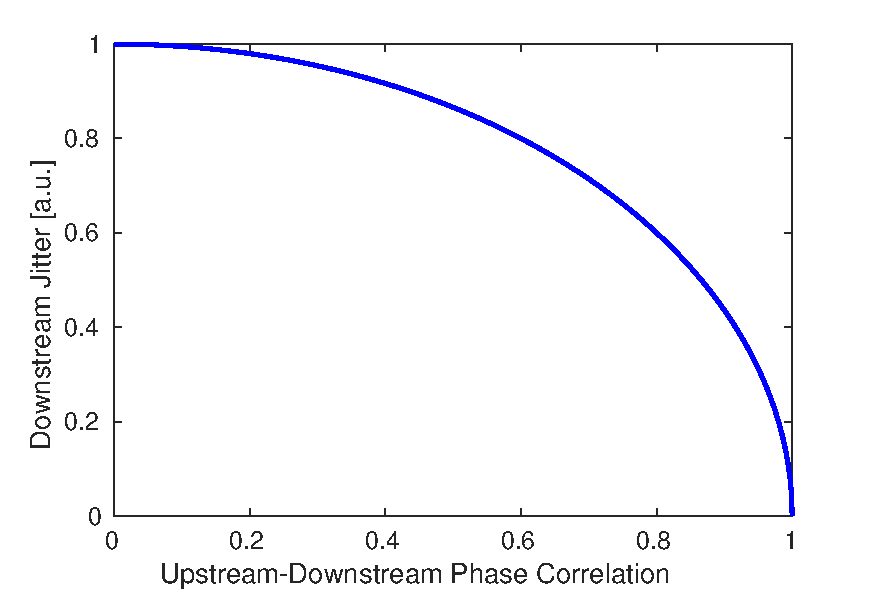
\includegraphics[width=0.8\textwidth]{Figures/propagation/theoretJitvsCorr}
  \caption{Dependence of the theoretical corrected downstream phase jitter on the initial upstream-downstream phase correlation, with an initial downstream phase jitter of 1~degree.}
  \label{f:theoretJitvsCorr}
\end{figure}

\newsection{origJitter}{Characteristics of Uncorrected Phase Jitter}

This section summarises the status of the phase propagation during the first PFF tests to demonstrate why the work in this chapter was necessary and to provide a point of comparison to the improved conditions later achieved in Section~\ref{s:bestPhaseProp}.

\subsubsection{Mean Phase}

Figure~\ref{f:origMeanPhJit} compares the mean phase upstream and downstream across one dataset of 213 pulses, or roughly 5 minutes. The downstream phase jitter is more than double the upstream phase jitter --- at \(1.86\pm0.09^\circ\) compared to \(0.81\pm0.04^\circ\) upstream. Theoretically the PFF system could still remove the amplified downstream phase jitter providing the jitter is still well correlated with the upstream phase, as derived in the previous section. Unfortunately, as shown in Figure~\ref{f:origUpVsDown}, there is only very weak correlation between the upstream and downstream phase, \(0.34\pm0.06\) in this case.

\begin{figure}
  \centering
  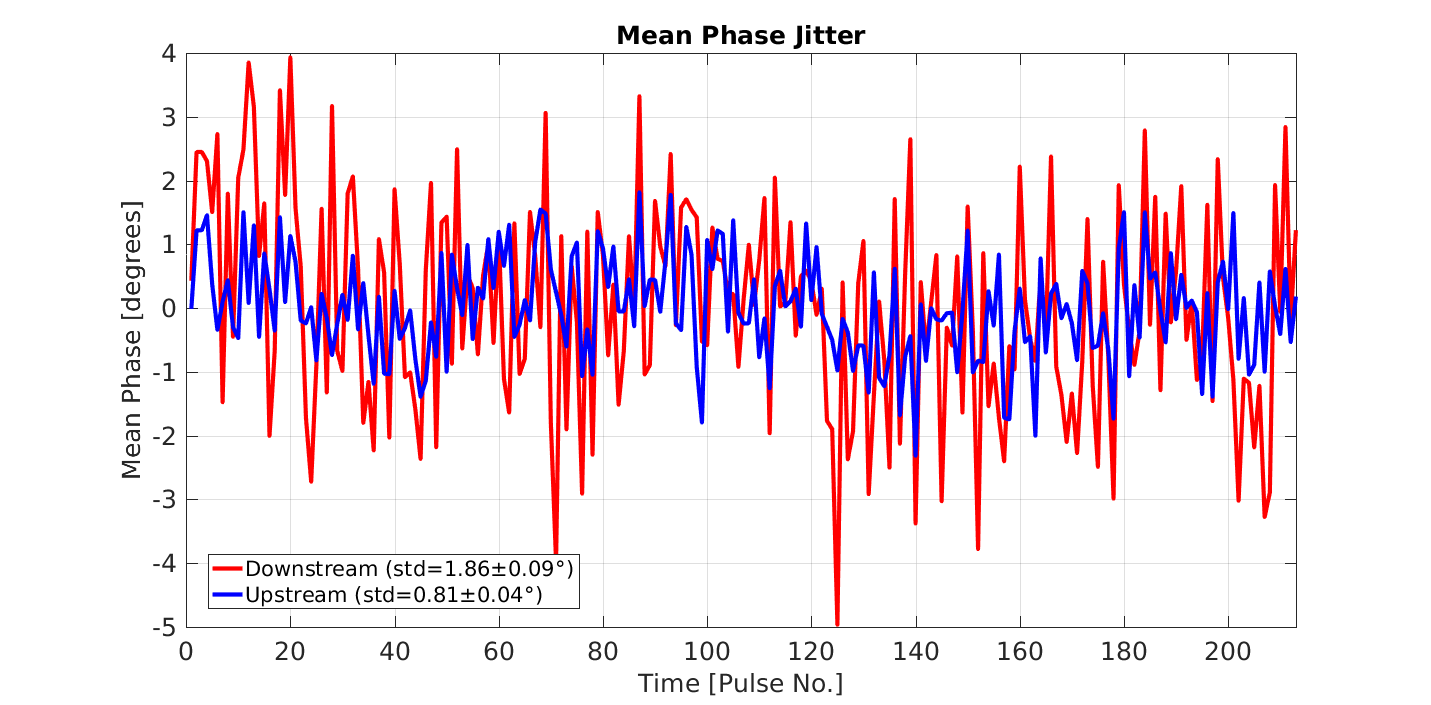
\includegraphics[width=0.9\textwidth]{Figures/propagation/origMeanPhJit}
  \caption{Mean phase jitter upstream (blue) and downstream (red) during early PFF tests.}
  \label{f:origMeanPhJit}
\end{figure}

\begin{figure}
  \centering
  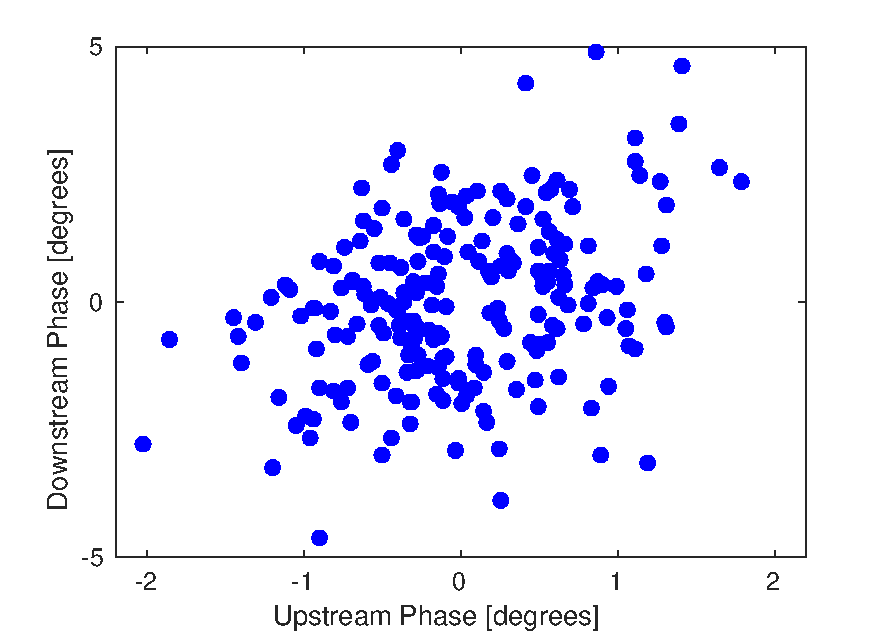
\includegraphics[width=0.8\textwidth]{Figures/propagation/origUpVsDown}
  \caption{Correlation between the downstream phase and the upstream phase during early PFF tests.}
  \label{f:origUpVsDown}
\end{figure}

Using Equation~\ref{e:theoretJitOptGain}, with the optimal PFF gain applied an initial downstream phase jitter of \(1.86\pm0.09^\circ\) could be reduced to \(1.51\pm0.09^\circ\) with the PFF system in these conditions with \(0.34\pm0.06\) upstream--downstream phase correlation. This is only a modest improvement of around 20\%, and far from the CLIC target of \(0.2^\circ\) phase stability. Also, the limitations of the actual PFF system, such as in the correction range (Section~\ref{ss:corrRange}), means that in reality even this 20\% reduction would be difficult to achieve in reality.

Assuming the downstream phase jitter could be reduced to the same level as the upstream phase jitter, at \(0.8^\circ\), the upstream--downstream phase correlation required to be able to make \(0.2^\circ\) corrected phase jitter theoretically possible is 97\%. The target of this chapter is to achieve both this correlation and downstream phase jitter.

\subsubsection{Phase Along Pulse}

In addition to the differences in the mean phase there are also large discrepancies between the upstream and downstream phase along the pulse. Figure~\ref{f:origPhaseAlong} shows one example of this. The overall phase sag along the pulse is approximately equivalent for both the upstream and downstream phase. However, there are many oscillations along the downstream phase, up to \(10^\circ\) peak-to-peak, that are not present upstream. Clearly these differences also need to be removed to enable phase jitters close to the CLIC target to be achieved with the PFF prototype at CTF3. 

\begin{figure}
  \centering
  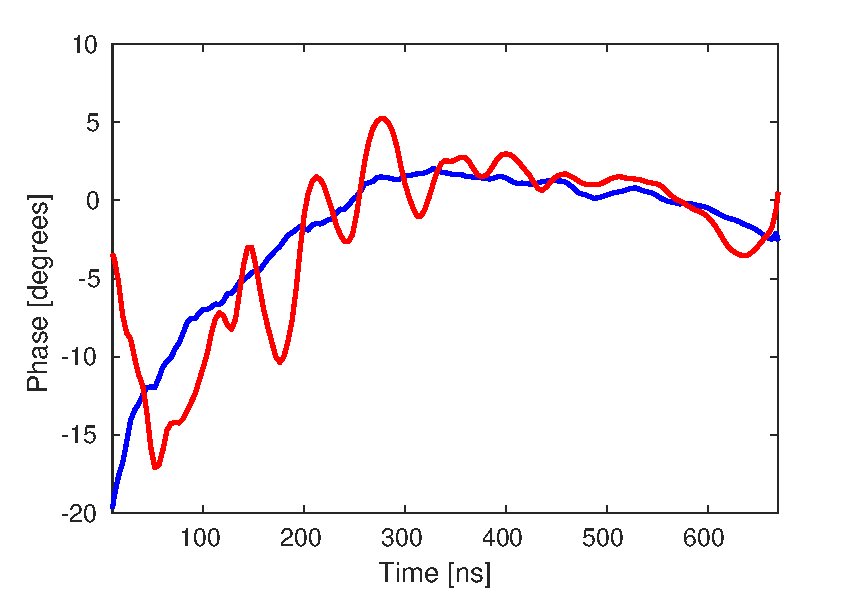
\includegraphics[width=0.8\textwidth]{Figures/propagation/origPhaseAlong}
  \caption{Upstream (blue) and downstream (red) phase along the pulse during early PFF tests.}
  \label{f:origPhaseAlong}
  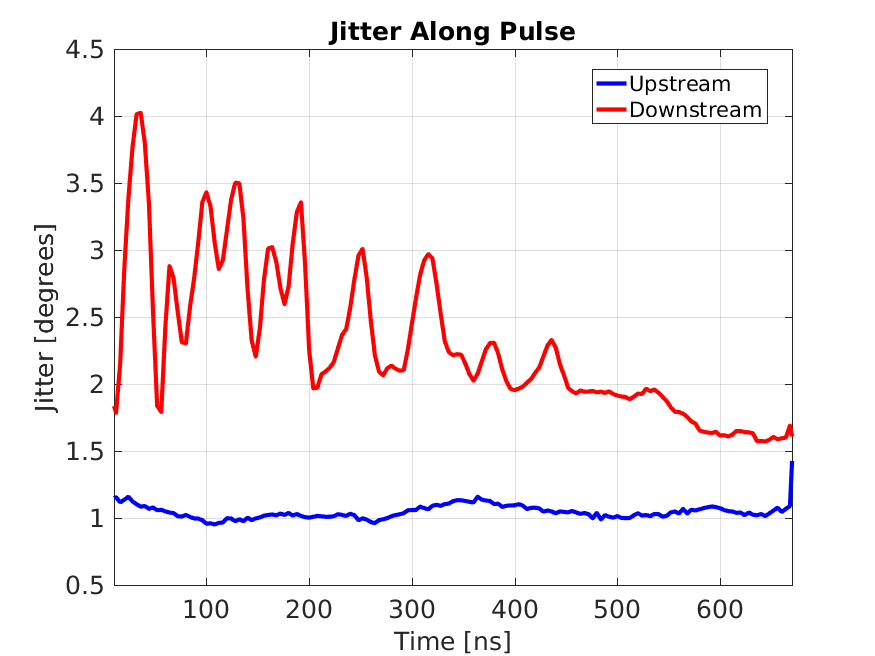
\includegraphics[width=0.8\textwidth]{Figures/propagation/origJitterAlong}
  \caption{Upstream (blue) and downstream (red) phase jitter along the pulse during early PFF tests.}
  \label{f:origJitterAlong}
\end{figure}


As well as the static variations in the downstream phase along the pulse, there are also large differences in the phase jitter along the pulse. This is shown in Figure~\ref{f:origJitterAlong}. The point by point upstream phase jitter along the pulse is quite flat at around 1 degree, slightly larger than the jitter on the mean. Alternatively, the downstream phase jitter has large variations in stability along the pulse. In some regions the downstream jitter is a factor 4 higher than the upstream phase jitter, whilst in others it is only 50\% higher.

\newsection{r56}{First Order Energy Dependencies}

The transfer matrix coefficient \(R_{56}\) defines the phase shift between two points in the lattice resulting from a beam energy offset (Section~\ref{c:opticsIntro}). Due to issues with meeting all the optics constraints for the PFF system a non-zero \(R_{56}\) value of close to -0.2~m had to be tolerated in the TL2 chicane (Section~\ref{ss:pffMatched}).  As a result a dependence of the downstream phase on the beam energy is expected. Naturally, this was the first place to look to try to understand and improve the poor upstream--downstream phase correlation and high downstream phase jitter.

\subsection{Beam Energy Variations}
\label{ss:energyVariations}

The best way to measure variations in the beam energy at CTF3 is via the beam position in one of the chicanes or rings, where the position after a bending magnet depends on the beam energy. The beam position offset, \(\Delta x\), in a BPM (beam position monitor) in these regions is linked to the relative energy offset, \(\Delta p / p\), as follows:
\begin{equation}
\frac{\Delta p}{p} = \frac{\Delta x}{D_x}
\end{equation}
Where \(D_{x}\) is the dispersion at that location given by the machine optics. Regions where \(D_{x}\) is non-zero are referred to as dispersive regions.

For the current beam setup used for the PFF system (bypassing the stretching chicane and delay loop, see Figure~\ref{f:ctfLayout}) the first dispersive BPM after the CTF3 linac is the BPM CT.0608 in the transfer line TL1.  TL1 is introduced in more detail in Section~\ref{ss:tl1Optics}. The BPM CT.0608 is placed roughly 1~m after the first dipole magnet in TL1, with a horizontal dispersion of \(D_{x} = -0.61\)~m at this point according to the CTF3 MADX model. There are no quadrupoles or other elements between the dipole and CT.0608, which reduces the sensitivity of this dispersion value to any inaccuracies in the model. All quoted energy measurements in this chapter are obtained using the horizontal position in BPM CT.0608, converted in to the energy using the equation above. %The only exception is Section~\ref{ss:corrPhaseEnergy}, as this includes measurements from an earlier setup where the stretching chicane was in use. A dispersive BPM in the stretching chicane, CT.0285, is used instead in that section but both BPMs give equivalent measured energies.

It should be noted that whilst this provides an accurate measurement of the relative energy jitter and variations along the pulse, it cannot be used to determine the absolute energy value. The mean beam position in CT.0608 is non-zero due to device misalignments, for example. This mean position offset is subtracted in all cases so that the resulting energy values are centred around zero, although the actual mean energy offset may be non-zero. In certain simulations in this chapter non-zero mean energy offsets are used to improve the agreement with the data, as indicated.

\subsubsection{Mean Beam Energy}

Figure~\ref{f:enJitter_mean} shows an example of variations in the mean beam energy on medium to long timescales at CTF3, in this case 500 pulses or roughly 10 minutes. Relative energy jitter on the mean is typically at the level of \(1 \times 10^{-3}\), and varies by roughly \(\pm50\%\) about this value. For shorter timescales, in datasets up to a couple of hundred pulses or a few minutes in length, the relative energy jitter is routinely closer to the \(0.5 \times 10^{-3}\) level (seen later in Figure~\ref{f:r56Scan_upstreamParams}, for example). The main sources of drifts in the mean energy at CTF3 are variations in beam current and temperature dependent effects on the klystron phase and RF power feedback loops \cite{lukasIPAC16}. Recent improvements have demonstrated below \(1 \times 10^{-3}\) energy stability also on longer timescales (see Section~\ref{ss:t566Mitigation}), which will aid future PFF tests.

\begin{figure}
  \centering
  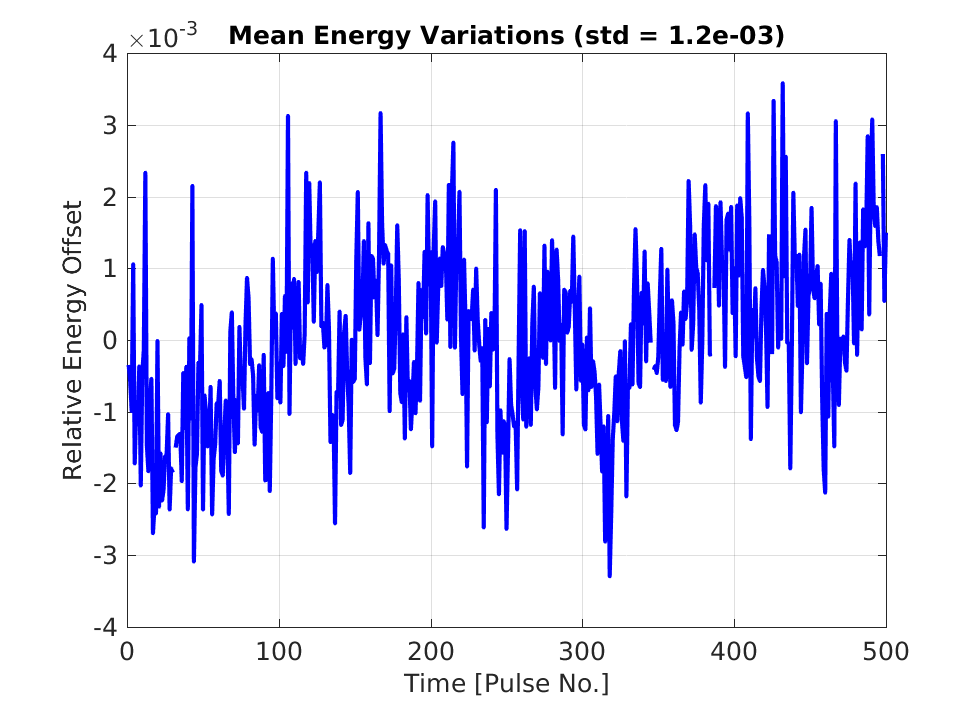
\includegraphics[width=0.8\textwidth]{Figures/propagation/enJitter_mean}
  \caption{Example of variations in mean energy across 500 pulses, with a relative jitter of \(1.2\times 10^{-3}\).}
  \label{f:enJitter_mean}
\end{figure}

\subsubsection{Energy Variations Along the Pulse}

Energy stability point by point along the pulse is at the same level as the mean energy stability, with relative jitter at, or slightly above, the \(1 \times 10^{-3}\) level, as seen in Figure~\ref{f:enJitter_along}. Typically the energy stability is slightly worse at the start and end of the pulse.

\begin{figure}
  \centering
  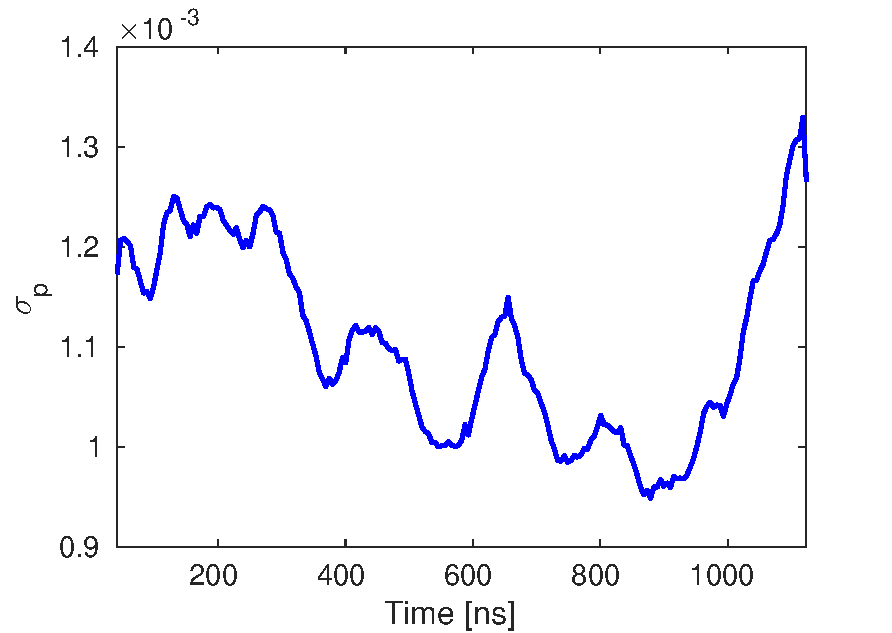
\includegraphics[width=0.8\textwidth]{Figures/propagation/enJitter_along}
  \caption{Example of relative energy jitter along the pulse.}
  \label{f:enJitter_along}
\end{figure}

In addition to the jitter there are also static variations in the energy along the pulse. Figure~\ref{f:enMeanAlong} shows one example of this. Peak-to-peak variations in the energy along the pulse are normally several times larger than the energy jitter, at the level of 2---\(5\times 10^{-3}\). New feedbacks have also been recently developed at CTF3 to reduce variations in energy along the pulse (Section~\ref{ss:t566Mitigation}).

\begin{figure}
  \centering
  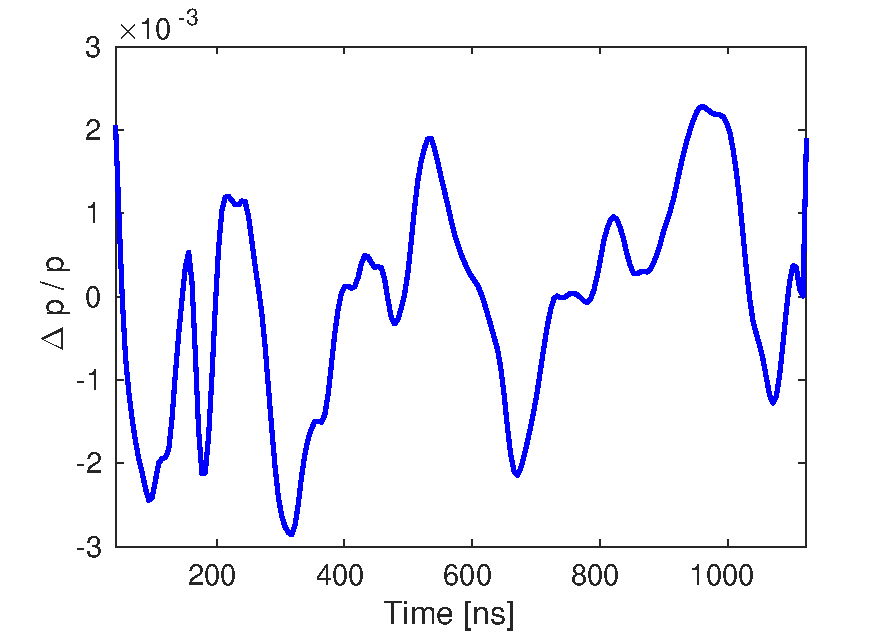
\includegraphics[width=0.8\textwidth]{Figures/propagation/enMeanAlong}
  \caption{Example of variations in energy along the pulse.}
  \label{f:enMeanAlong}
\end{figure}


\subsection{Correlation between Phase and Energy}
\label{ss:corrPhaseEnergy}

Figure~\ref{f:corrDownstream_En} shows one example of the typical dependence of the mean downstream phase on the beam energy during the first PFF attempts. It's immediately clear that there is a strong relationship between the two, with a correlation in this case of \(0.82\pm0.03\). 

Alternatively, in Figure~\ref{f:corrUpstream_En} there is almost no dependence of the upstream phase on the energy. However, the calculated correlation coefficient of \(0.19\pm0.06\) is statistically significant and this has consequences for the discussions in the remainder of this chapter. Normally the small upstream phase--energy correlation typically varies between 0 and 0.4 at CTF3 depending on the conditions, in particular the energy jitter, at that time. In certain setups there can also be high correlations between the upstream phase and energy (Section~\ref{s:r56ScanWithEnergy}).

By itself having a high correlation between the downstream phase and the energy is not an issue for the PFF system. The problem is the difference between the upstream phase--energy correlation and the downstream phase--energy correlation, which leads to low correlation between the upstream and downstream phase. The high downstream phase jitter is also a problem for the PFF system due to its limited correction range, as previously mentioned.

The goal of this section is to determine whether the non-zero optics \(R_{56}\) value between the upstream and downstream phase monitors is sufficient to explain both the large amplification in downstream phase jitter and the low upstream--downstream phase correlation seen here. To start, the effect of \(R_{56}\) on the downstream phase jitter and upstream--downstream phase correlation will be more formally defined.

\begin{figure}
  \centering
  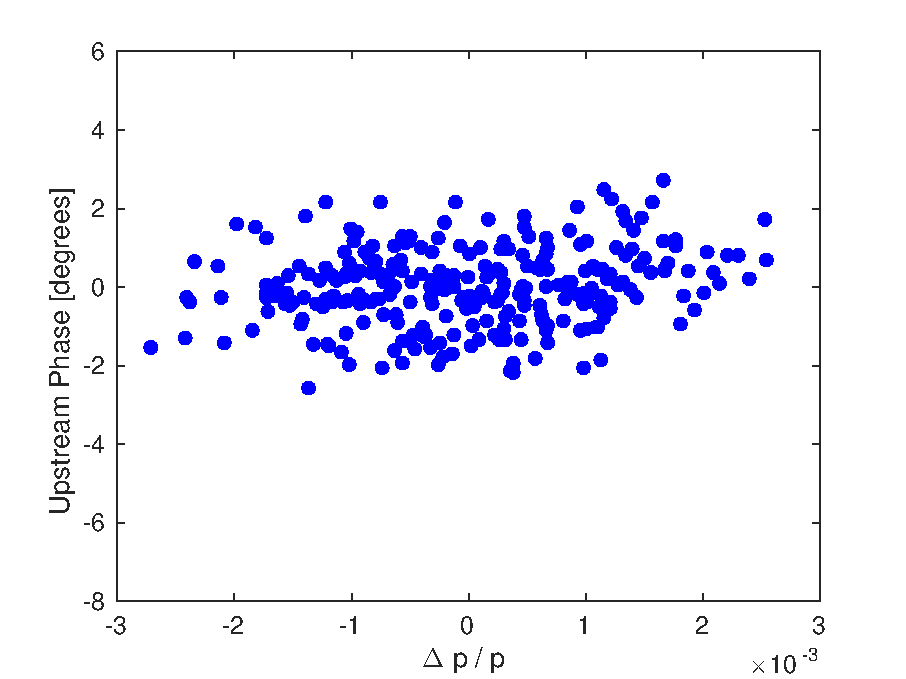
\includegraphics[width=0.8\textwidth]{Figures/propagation/corrUpstreamEn}
  \caption{Dependence of the mean upstream phase on the beam energy.}
  \label{f:corrUpstream_En}
\end{figure}

\begin{figure}
  \centering
  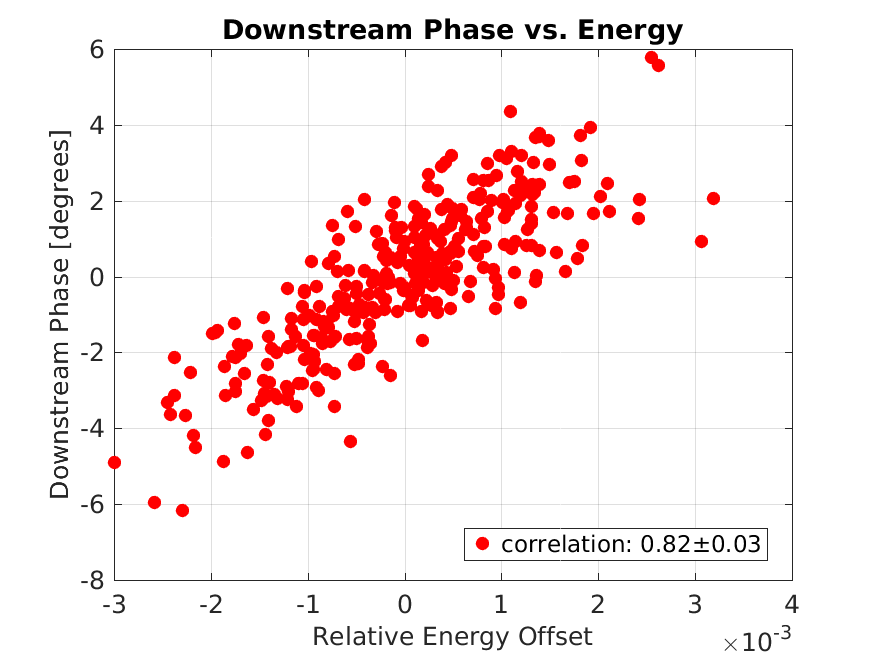
\includegraphics[width=0.8\textwidth]{Figures/propagation/corrDownstreamEn}
  \caption{Dependence of the mean downstream phase on the beam energy.}
  \label{f:corrDownstream_En}
\end{figure}



\subsection{R56}
\label{ss:r56Equations}

Assuming energy is the only source of differences between the upstream and downstream phase, the downstream phase, \(\phi_d\), can be expressed in terms of the optics transfer matrix coefficient \(R_{56}\) (Section~\ref{s:opticsIntro}) as follows:
\begin{equation}
\phi_d = \phi_u + R_{56}\frac{\Delta p}{p}
\label{e:r56PhasEq}
\end{equation}

Where \(\phi_u\) is the upstream phase, \(\Delta p / p\) is the relative energy offset and \(R_{56}\) is the R56 value between the upstream and downstream phase monitors, defined by the machine optics. The units of R56 in the equation above are 12~GHz radians per unit relative energy offset (\(\Delta p/p = 1\)). MADX uses units of metres and this value is what will be referred to in this chapter. To obtain the R56 value to use in the equation above the MADX value must be multiplied by the conversion factor \(2\pi/0.025\), where 0.025~m is the 12~GHz wavelength.

In terms of jitters Equation~\ref{e:r56PhasEq} becomes:
\begin{equation}
\sigma_d = \sqrt{\sigma_u^2 + R_{56}^2\sigma_{p}^2 + 2R_{56}\rho_{up}\sigma_{u}\sigma_{p}}
\label{e:r56JitEq}
\end{equation}
Where \(\sigma_d\) is the downstream phase jitter, \(\sigma_u\) is the upstream phase jitter, \(\sigma_p\) is the relative energy jitter and \(\rho_{up}\) is the correlation between the upstream phase and the energy. This follows from the result of adding correlated variances. Clearly, any non-zero R56 between the upstream and downstream phase monitors introduces an additional energy component to the downstream phase that increases the downstream phase jitter.

The effect of R56 on the upstream-downstream phase correlation, \(\rho_{ud}\), can also be defined starting from the definition of the correlation coefficient:
\begin{equation}
\rho_{ud} = \frac{\mathrm{cov}\left[\phi_u,\phi_d\right]}{\sigma_u\sigma_d}
\label{e:r56CorrDef1}
\end{equation}
Where \(\mathrm{cov}\left[\phi_u,\phi_d\right]\) is the covariance between the upstream and downstream phase, given by:
\begin{equation}
 \mathrm{cov}\left[\phi_u,\phi_d\right] = \frac{1}{N} \sum_{i=1}^{N}\phi_{ui}\phi_{di}
\label{e:r56CorrDef2}
\end{equation} 
By inserting the definition of the downstream phase from Equation~\ref{e:r56PhasEq} and separating the terms in the sum this becomes:
\begin{equation}
\mathrm{cov}\left[\phi_u,\phi_d\right] = \frac{1}{N} \sum_{i=1}^{N}\phi_{ui}^{2} + R_{56}\frac{1}{N} \sum_{i=1}^{N}\phi_{ui}\frac{\Delta p}{p}
\label{e:r56CorrDef3}
\end{equation}
The first term is now the variance of the upstream phase, \(\sigma_u^2\), and the second term is \(R_{56}\) multiplied by the covariance between the upstream phase and the energy, \(\mathrm{cov}\left[\phi_u,\frac{\Delta p}{p}\right]\), which can be expressed in terms of the correlation between the upstream phase and the energy, \(\rho_{up}\):
\begin{equation}
\mathrm{cov}\left[\phi_u,\frac{\Delta p}{p}\right] = \rho_{up}\sigma_u\sigma_{p}
\label{e:r56CorrDef4}
\end{equation}
Therefore, Equation~\ref{e:r56CorrDef3} becomes:
\begin{equation}
\mathrm{cov}\left[\phi_u,\phi_d\right] = \sigma_u^2 + R_{56}\rho_{up}\sigma_u\sigma_p
\label{e:r56CorrDef5}
\end{equation}
Finally, substituting Equations~\ref{e:r56JitEq}~and~\ref{e:r56CorrDef5} into Equation~\ref{e:r56CorrDef1} gives:
\begin{equation}
\rho_{ud} = \frac{\sigma_u + R_{56}\rho_{up}\sigma_p}{\sqrt{\sigma_u^2 + R_{56}^2\sigma_{p}^2 + 2R_{56}\rho_{up}\sigma_{u}\sigma_{p}}}
\label{e:r56CorrDefFinal}
\end{equation}

Considering that in this model the only difference between the upstream and downstream phase results from the R56, it is perhaps obvious that the best conditions for the PFF correction are obtained when the R56 coefficient between the upstream and downstream phase monitors is zero. In these conditions \(\sigma_d = \sigma_u\) and \(\rho_{ud} = 1\). This can be more formally defined by using the expression for the theoretical corrected downstream phase jitter when using the optimal gain factor as derived in Section~\ref{ss:theoryJitter}:
\begin{equation}
\sigma_{PFF} = \sigma_d\sqrt{1-\rho_{ud}^2}
\end{equation}
All these quantities have been derived above and inserting them in to this equation gives the following expression for the corrected downstream phase jitter in terms of the R56:
\begin{equation}
\sigma_{PFF} = \left|R_{56}\right|\sigma_p\sqrt{1-\rho_{up}^2}
\label{e:r56PFFJit}
\end{equation}
As expected the achievable corrected downstream phase jitter is minimised when \(R_{56}~=~0\). Note that this equation does not take in to account that the minimum achievable downstream phase jitter is limited to \(\sqrt{2}\) times the phase monitor resolution [REF].

In principle, the beam conditions for the PFF correction can also be improved by reducing the relative energy jitter (\(\sigma_p\)) or by increasing the upstream phase-energy correlation (\(\rho_{up}\)). Reducing the relative energy jitter decreases the additional phase jitter created by non-zero R56. Increasing the upstream phase-energy correlation (\(\rho_{up}\)) reduces the effect that non-zero R56 has on the upstream-downstream phase correlation (\(\rho_{ud}\)). For example, if \(\rho_{up}=1\) the source of all upstream phase jitter is energy jitter. In that case although non-zero R56 would further increase the downstream phase jitter, the additional jitter would be well correlated with the upstream phase and the upstream-downstream phase correlation would not be affected. In practice \(\sigma_p\) and \(\rho_{up}\) are defined by the CTF3 injector and can not be varied with a great degree of flexibility, so having zero R56 is the only way to obtain ideal conditions for the PFF correction. However, recent improvements at CTF3 have reduced the relative energy jitter, as discussed later in Section~\ref{ss:t566Mitigation}. High upstream phase-energy correlations can also be created at CTF3 but not without greatly amplifying the upstream phase jitter, which causes issues for the PFF system due to its limited correction range (Section~\ref{s:pffNovelSetups}).

An interesting side note of Equations~\ref{e:r56JitEq}~and~\ref{e:r56PFFJit} is that the best beam conditions for the PFF correction are not given by minimising the initial downstream phase jitter in the case where the upstream phase-energy correlation, \(\rho_{up}\), is non-zero. As seen in the previous section in normal conditions there is a small correlation between the upstream phase and the energy at CTF3, typically around \(\rho_{up}=0.2\). In these conditions the downstream phase jitter can in theory be reduced to below the level of the upstream phase jitter by using a negative R56 to remove the energy component in the downstream phase. Differentiating Equation~\ref{e:r56JitEq} gives the minimum downstream phase jitter to be obtained when \(R_{56} = -\rho_{up}\sigma_u/\sigma_p\). However, using this \(R_{56}\) value would degrade the upstream-downstream phase correlation and increase the achievable corrected downstream jitter, which is always minimised when \(R_{56} = 0\) as in Equation~\ref{e:r56PFFJit}. This is significant for the \(R_{56}\) optimisation attempts presented later in this chapter, as it must always be kept in mind that the goal is to maximise the upstream-downstream phase correlation rather than to create the most stable downstream phase (with the PFF system off).

\subsection{Effect of R56 in TL2}
\label{ss:r56TL2Effect}

Unfortunately, it was not possible to find optics for the TL2 chicane that met all the PFF requirements and thus an R56 in the chicane of close to -0.2~m had to be accepeted (Section~\ref{ss:pffMatched}). All other lines at CTF3 nominally have zero R56 \cite{CTF3}, and therefore don't introduce additional phase jitter via energy, at least to first order and to within the accuracy of the CTF3 MADX model. The overall R56 between the upstream phase monitors (in the CT line) and the downstream phase monitors (in the TBL line, labelled CB, after the TL2 chicane) is therefore -0.2~m also. Whether this can explain the low upstream-downstream phase correlation and high downstream phase jitter seen in Section~\ref{s:origJitter}, as well as what residual R56 between the two monitors can be tolerated to be able to achieve CLIC-level phase stability at CTF3, is discussed in this section.

Equations~\ref{e:r56JitEq}~and~\ref{e:r56CorrDefFinal} can be used to estimate the downstream phase jitter and upstream-downstream phase correlation in the conditions at CTF3. Typical values for the various parameters in the equations have already been presented in previous sections, and these values are summarised in Table~\ref{t:r56Params}. The value \(R_{56}\simeq -0.2\) was obtained in Section~\ref{ss:pffMatched} as previously mentioned, the value \(\sigma_u\simeq0.8^\circ\) in Section~\ref{s:origJitter} and the values \(\rho_{up}\simeq 0.2\) and \(\sigma_p\simeq 0.001\) in Section~\ref{ss:corrPhaseEnergy}.

\begin{table}
  \begin{center}
    \begin{tabular}{| c c |}
	   \hline
       Parameter & Value \\ \hline
       \(R_{56}\) & -0.2~m \\
       \(\sigma_u\) & \(0.8^\circ\) \\
       \(\rho_{up}\) & 0.2 \\
       \(\sigma_{p}\) & 0.001 \\ \hline
    \end{tabular}
    \caption{Typical upstream phase and energy conditions at CTF3.}
  	\label{t:r56Params}
  \end{center}
\end{table}

With these parameter values the residual R56 of -0.2~m reduces the upstream-downstream phase correlation to below 10\%, and amplifies the downstream phase jitter to above 3~degrees. Therefore, R56 transforming energy jitter in to downstream phase jitter can by itself explain the low upstream-downstream phase correlation and high downstream phase jitter seen in Section~\ref{s:origJitter}. In order to increase the upstream-downstream phase correlation to 97\% and reduce the downstream jitter to 0.8~degrees (the conditions needed to achieve 0.2~degrees corrected downstream phase jitter at CTF3) the R56 between the upstream and downstream phase monitors must be removed.

Figure~\ref{f:jitVsR56}~and~\ref{f:corrVsR56} show the expected downstream phase jitter and upstream-downstream phase correlation for residual R56 values from -0.2 to +0.2~m between the upstream and downstream phase monitors again using the equations derived in the previous section. The horizontal black line in each figure marks the requirements needed to reduce an initial upstream phase jitter of 0.8 degrees to the CLIC target of 0.2 degrees. The red line, "corrected", in Figure~\ref{f:jitVsR56} shows the theoretical corrected downstream phase jitter using the PFF correction across the range of R56 values. Note the slight asymmetry in the phase jitter and correlation curves, which is caused by the non-zero correlation between the upstream phase and the beam energy. In order to obtain CLIC level phase stability at CTF3 the residual R56 between the upstream and downstream phase monitors must be reduced from the initial \(-0.2m\) to \(0\pm1.3~cm\).

\begin{figure}
  \centering
  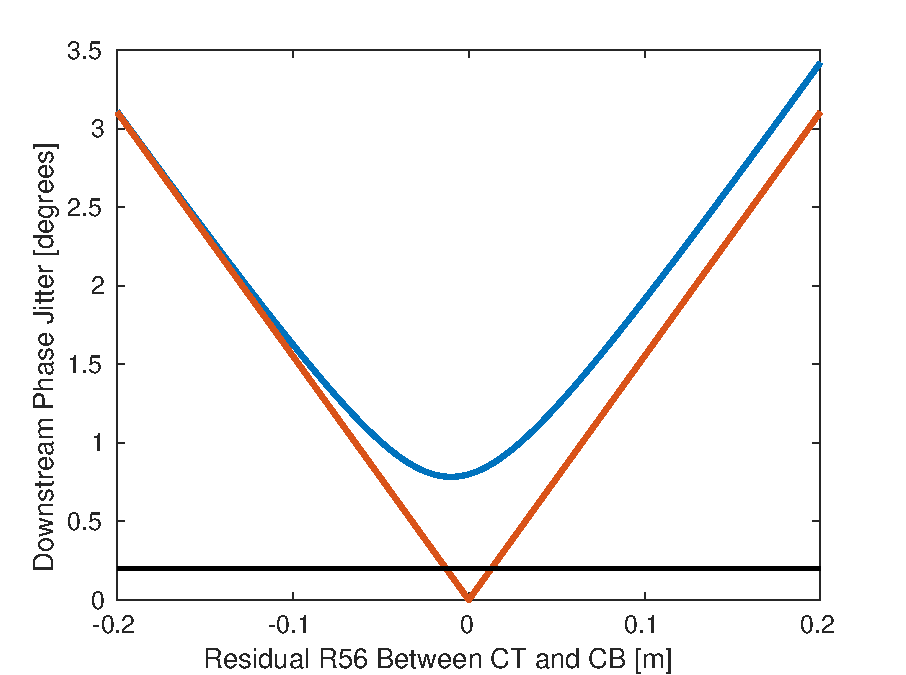
\includegraphics[width=0.8\textwidth]{Figures/propagation/jitVsR56}
  \caption{Initial (blue) and corrected (red) downstream phase jitter vs. the \(R_{56}\) coefficient between the upstream and downstream phase monitors. The horizontal black line shows the CLIC target of 0.2~degrees corrected downstream phase jitter.}
  \label{f:jitVsR56}
  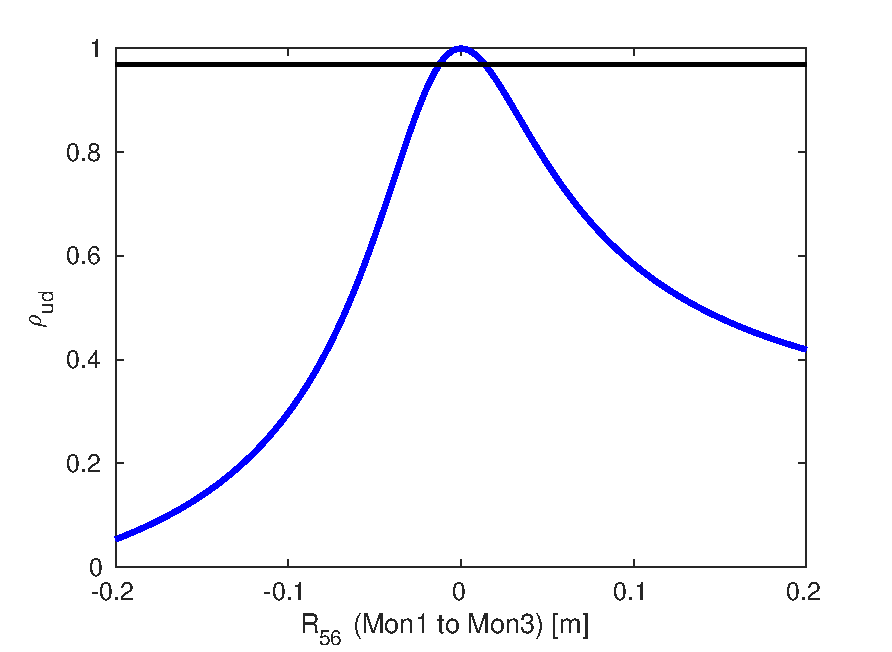
\includegraphics[width=0.8\textwidth]{Figures/propagation/corrVsR56}
  \caption{Upstream-downstream phase correlation vs. the \(R_{56}\) coefficient between the upstream and downstream phase monitors. The horizontal black line shows the 97\% correlation needed to achieve 0.2~degrees corrected phase jitter at CTF3.}
  \label{f:corrVsR56}
\end{figure}

To interpret the results of the R56 optimisation attempts presented in the remainder of this chapter it is useful to understand how varying the correlation between the usptream phase and the energy (\(\rho_{up}\) changes the dependence of the upstream-downstream phase correlation (\(\rho_{ud}\)) on the residual R56. In particular, in Section~\ref{ss:r56ScanWithEnergy} a machine setup that increases \(\rho_{up}\) to 90\% was used. Figure~\ref{f:corrVsR56_CTENCorr} shows how \(\rho_{ud}\) varies with \(\rho_{up}\) values between 0\% and 40\% (typical of normal operation) and with the higher correlation of 90\%. With high correlations between the upstream phase and energy there is no longer a well defined peak in \(\rho_{ud}\) versus the residual R56 value. Instead there is an almost constant high upstream-downstream phase correlation with positive R56 values, and a large anti-correlation for negative R56 values (as in this case the residual R56 acts to flip the sign of the phase jitter). 

\begin{figure}
  \centering
  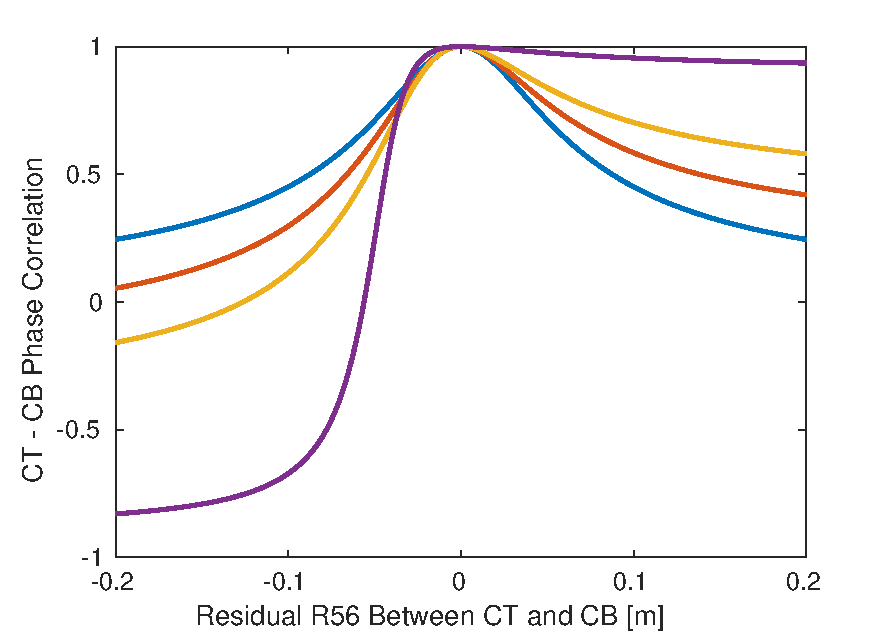
\includegraphics[width=0.8\textwidth]{Figures/propagation/corrVsR56_CTENCorr}
  \caption{Upstream-downstream phase correlation (\(\rho_{ud}\)) vs. the \(R_{56}\) coefficient between the upstream and downstream phase monitors for different upstream phase-energy correlations: \(rho_{up}=0.0\) (blue), \(rho_{up}=0.2\) (red), \(rho_{up}=0.4\) (orange) and \(rho_{up}=0.9\) (purple).}
  \label{f:corrVsR56_CTENCorr}
  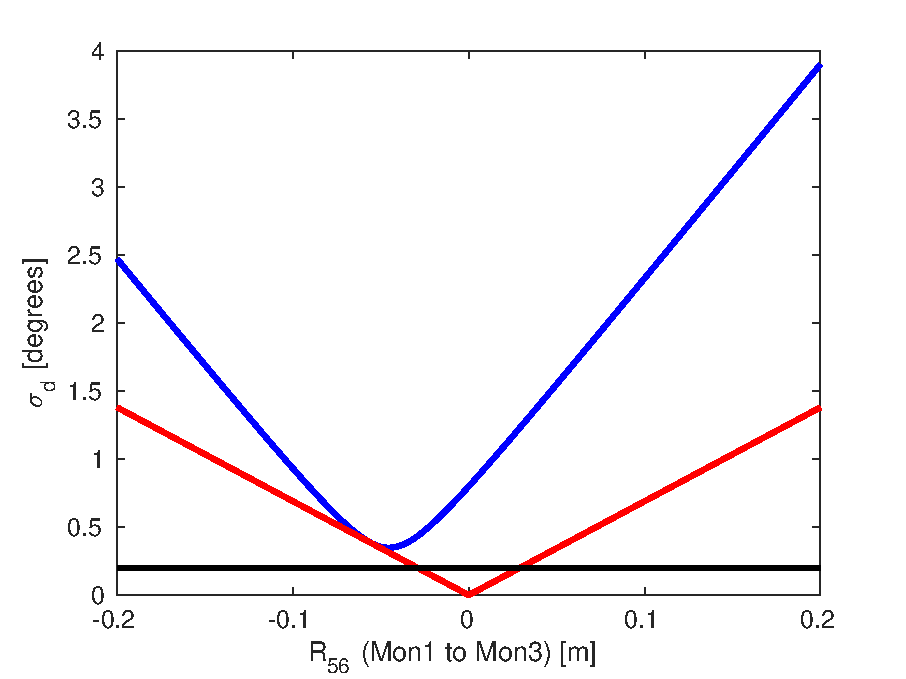
\includegraphics[width=0.8\textwidth]{Figures/propagation/jitVsR56_90ctencorr}
  \caption{Initial (blue) and corrected (red) downstream phase jitter vs. the \(R_{56}\) coefficient between the upstream and downstream phase monitors with 90\% correlation between the upstream phase and the beam energy.}
  \label{f:jitVsR56_90ctencorr}
\end{figure}


In Figure~\ref{f:jitVsR56_90ctencorr} plotting the theoretical downstream jitter with \(\rho_{up} = 0.9\) gives a clear demonstration that the best conditions for the PFF correction are always with \(R_{56} = 0\) rather than with the lowest possible initial downstream jitter, as mentioned in the previous section. In fact, as these conditions relax the requirements on the residual R56 needed to achieve high upstream-downstream phase correlations (as seen in the previous figure) it may be easier to achieve a large factor reduction in the downstream phase jitter with the PFF system with a high \(\rho_{up}\) machine setup. This has been attempted and is presented in Section~\ref{s:pffNovelSetups}.


\newsection{r56Removal}{Mitigation of First Order Energy Dependence}

The discussion in the previous section proves that with a residual R56 value of -0.2~m between the upstream and downstream phase monitors it is impossible to achieve the goals of the PFF prototype at CTF3. However, due to the highly constrained optics in TL2 it has already been seen in Chapter~\ref{c:tl2Optics} that it was not possible to find optics for the PFF chicane that yield zero R56 whilst also meeting requirements for both the PFF system and transverse matching (dispersion and beta functions). The only way to create a total R56 of zero between the upstream and downstream phase monitors is therefore to add positive R56 to one of the other beam lines at CTF3 in order to compensate for the negative R56 in the TL2 chicane. 

The previous transfer line TL1, which transports the beam from the CT line (where the upstream phase monitors are installed) to the combiner ring (see Figure~\ref{f:ctfLayout}), has been used to achieve this. The layout of the TL1 transfer line is shown in Figure~\ref{f:tl1Layout}. It consists of: 4 dipoles (bending the beam horizontally) of 2 different types, 13 quadrupoles of 5 different types, 7 magnetic correctors, 1 sextupole (usually not used) and 8 BPMs (the dispersive BPM after the first dipole in TL1, labelled CT.BPI0608, is the device that has been used to determine correlations between the phase and energy in this chapter). The total length of TL1 is approximately 30~m.

Preliminary attempts to reduce the residual R56 between the upstream and downstream phase monitors using TL1 yielded correlations up to 60\% and reduced the downstream phase jitter to \(2^\circ\). Conditions similar to these were used for the first PFF tests (Chapter~\ref{c:earlyFFSim}) before the energy related effects discussed in this chapter were fully characterised, but in these tests only a modest reduction of 30\% in downstream phase jitter was possible due to the limitations of the phase propagation shown here. At this time only a few different optics for TL1 were available in R56 steps of 10~cm. As the total residual R56 must be reduced to the centimetre level to make a correction down to 0.2 degrees jitter theoretically possible with the PFF system, new sets of optics for TL1 were required.

\afterpage{\begin{landscape}
	\begin{figure}
  		\centering
  		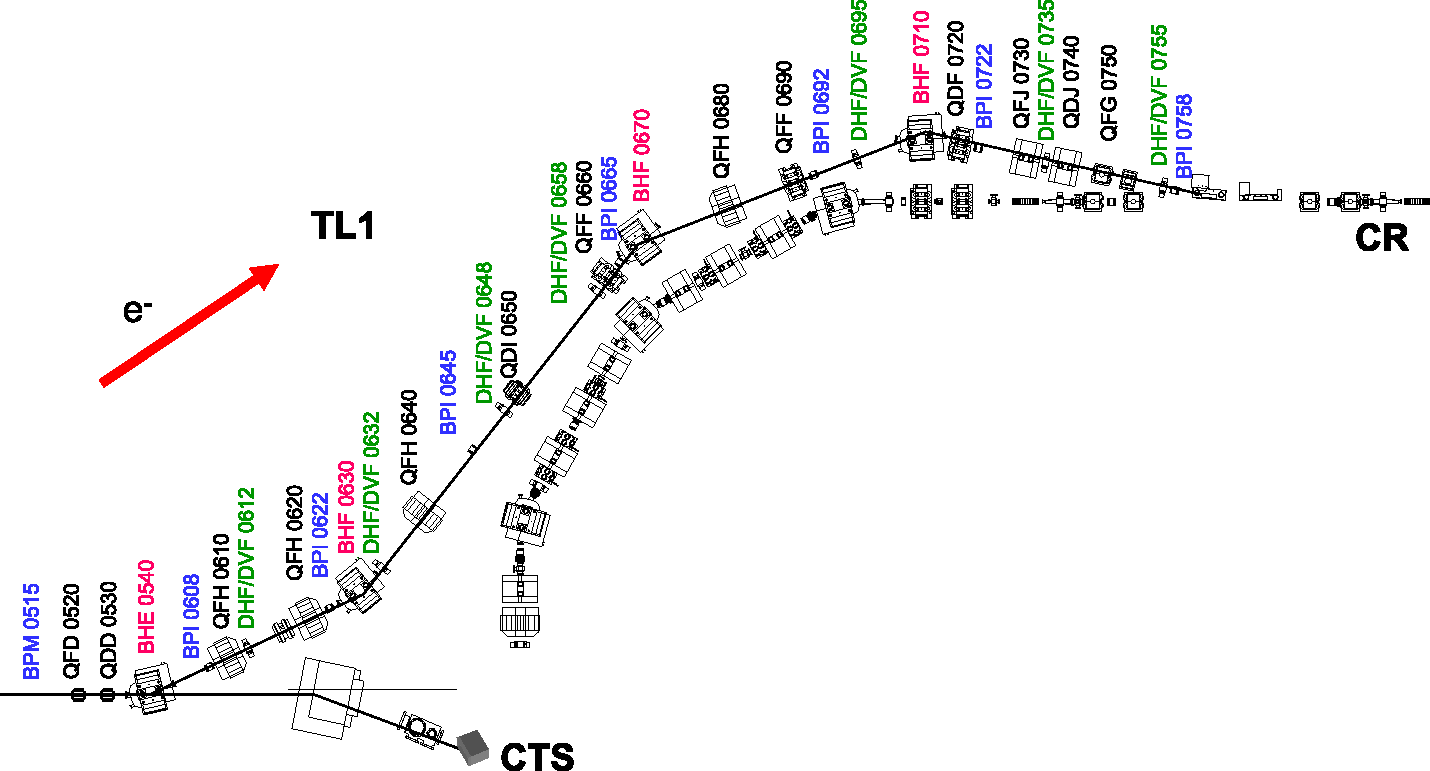
\includegraphics[height=\textwidth]{Figures/propagation/TL1}
  		\caption{Layout of dipoles, quadrupoles and BPMs in the TL1 transfer line \cite{tl1Layout}.}
  		\label{f:tl1Layout}
	\end{figure}
\end{landscape}}

\subsection{Matched Optics for TL1}
\label{ss:tl1Optics}

Although in theory only one set of optics with \(R_{56} = +0.2\)~m in TL1 is required to compensate for the \(R_{56} = -0.2\)~m in TL2, in practice errors in the MADX model of CTF3 plus the effect of higher order energy dependencies (see Section~\ref{s:t566}) means it is not possible to know precisely what the optimal R56 to set in TL1 will be, and it is also possible that this value will vary with time. To determine the optimal value of R56 to set it is also useful to scan the R56 value in TL1 across a wide range of values and then fit the maximum resulting upstream-downstream phase correlation.

To allow this, MADX has been used to match optics for TL1 with R56 values ranging from -0.3~m to +0.6~m in steps of 0.5~cm (a total of 181 sets of optics). The optimal R56 value should always be guaranteed to be in this range, and the step size of 0.5~cm allows the residual R56 to be zeroed to within one centimetre as derived to be necessary in Section~\ref{ss:r56TL2Effect}. As well as the different R56 values, each set of optics must maintain the same initial and final conditions, so that the injection of the beam in to the combiner ring is not affected. Values for the beta functions, alphas and dispersion at the start of TL1 and at the combiner ring injection are summarised in Table~\ref{t:tl1MatchParams}. As well as the initial and final conditions, the maximum beta functions and dispersion in TL1 are constrained to ensure a reasonable beam size throughout the line --- the horizontal and vertical beta function is limited to a maximum of 35~m, and the horizontal dispersion to a maximum absolute value of 1.25~m. Around the septum used for injection in to the combiner ring the horizontal beta function is further limited to a maximum of 10~m. The strengths of the 13 quadrupoles in TL1 are varied to meet all these constraints.

\begin{table}
  \begin{center}
    \begin{tabular}{| c c c |}
	   \hline
       Parameter & TL1 Injection & CR Injection \\ \hline
       \(\beta_x\) & 8.81~m & 4.08~m \\
       \(\beta_y\) & 13.94~m & 5.41~m \\
       \(\alpha_x\) & -0.74 & -0.31 \\
       \(\alpha_y\) & -0.45 & -0.21 \\ 
       \(D_x\) & 0~m & -0.03~m \\ 
       \(D_{px}\) & 0 & 0.02 \\ \hline
    \end{tabular}
    \caption{Initial and final conditions for optics matching in TL1.}
  	\label{t:tl1MatchParams}
  \end{center}
\end{table}

Figures~\ref{f:r56MatchedVsTarget} shows the matched R56 value in TL1 across the range of targeted values. Each matched R56 value is within 10 microns of the desired result. Figure~\ref{f:CTQFG0750} then shows an example of how the strength of one of the quadrupoles must be varied in order to achieve each R56 value. If the dependence of each quadrupole strength on the R56 value was continuous the relationship could be fitted to create a set of tuning knobs to allow R56 to be set to any arbitrary value in TL1. However, as seen in the figure there are many discontinuities. The quadrupole strengths for each set of optics are therefore saved to a lookup table, with a MatLab function created to read the table and set the quadrupole currents in the machine appropriate for the specified R56 value. As already mentioned 0.5~cm precision in R56 should be adequate for the PFF requirements, but the discontinuities mean new optics would have to be matched if optics with an R56 value not included in the discrete set used here were required.

\begin{figure}
  \centering
  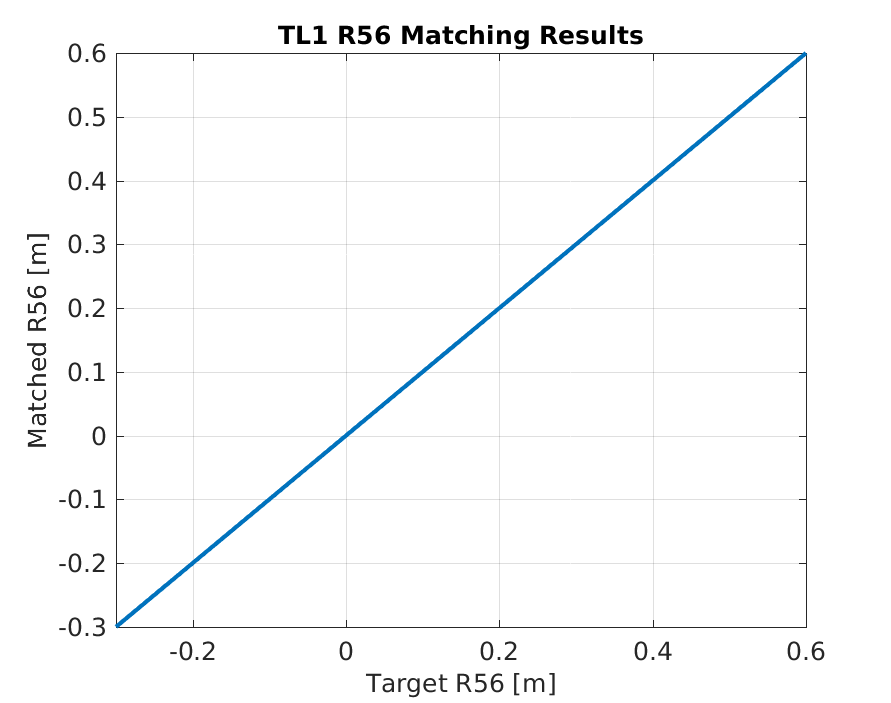
\includegraphics[width=0.8\textwidth]{Figures/propagation/r56MatchedVsTarget}
  \caption{Matched \(R_{56}\) values for the new sets of TL1 optics.}
  \label{f:r56MatchedVsTarget}
\end{figure}

\begin{figure}
  \centering
  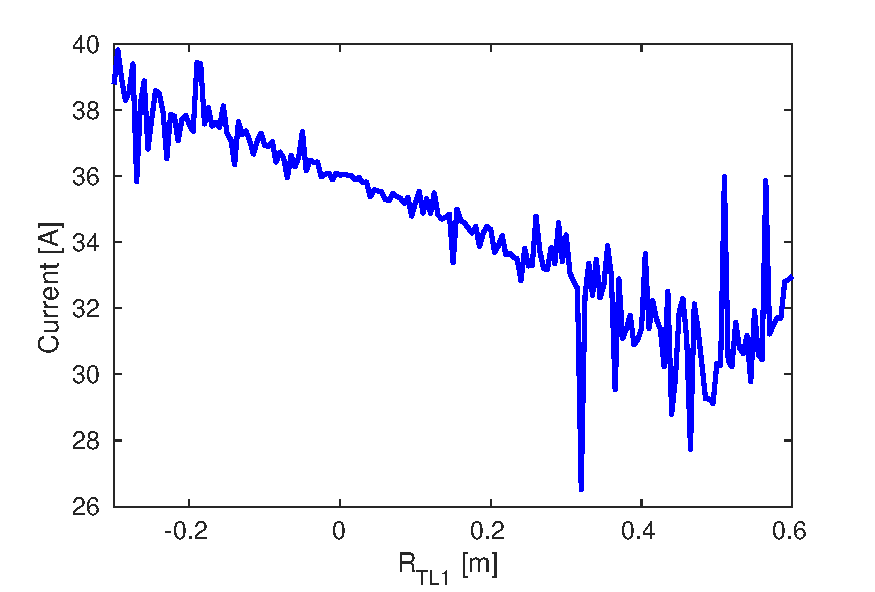
\includegraphics[width=0.8\textwidth]{Figures/propagation/CTQFG0750}
  \caption{Strength (power supply current) of the CT.QFG0750 quadrupole in TL1 vs. the \(R_{56}\) value in TL1 for each set of matched optics.}
  \label{f:CTQFG0750}
\end{figure}

For reference Figures~\ref{f:tl1BETX}~\ref{f:tl1BETY}~and~\ref{f:tl1DX} show how the horizontal and vertical beta functions and horizontal dispersion changes in TL1 for each set of optics. For all R56 values each parameter converges to the same value at the start and end of TL1, as needed to ensure that changing the R56 does not impact injection in to the combiner ring. The maximum horizontal and vertical beta functions in TL1 roughly increase with the set R56 value, but in all cases are kept below the set limit of 35~m in the matching procedure. The dispersion pattern in TL1 also changes with the set R56 value, though in most cases the maximum absolute dispersion is around 1~m and only the location of the peak dispersion along the line changes. Again, for each set of optics the maximum absolute dispersion is limited within the set constraint of 1.25~m. 

\begin{figure}
  \centering
  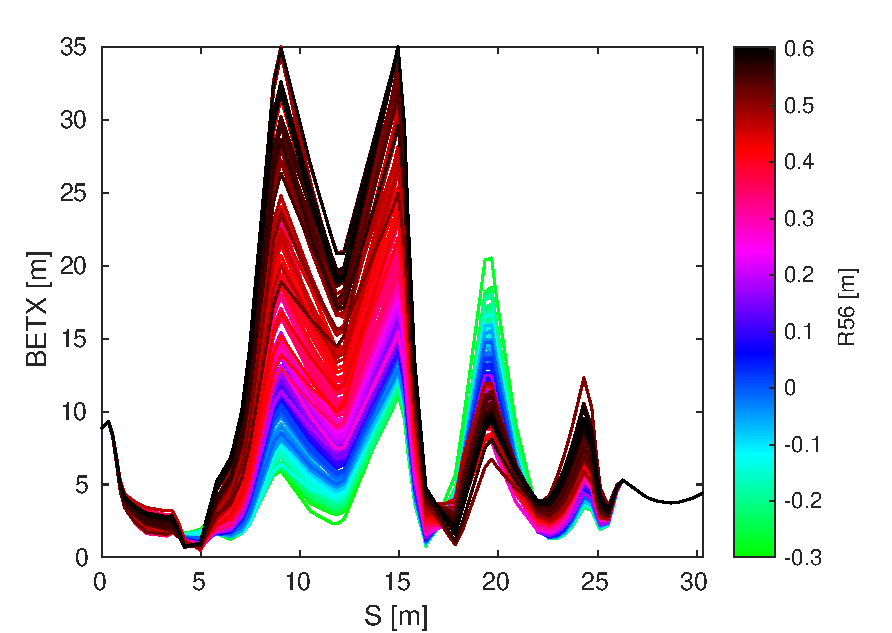
\includegraphics[width=0.8\textwidth]{Figures/propagation/BETX}
  \caption{Horizontal beta function in each set of optics for TL1, with the colour scale indicating the \(R_{56}\) value in TL1 for that optics.}
  \label{f:tl1BETX}
\end{figure}

\begin{figure}
  \centering
  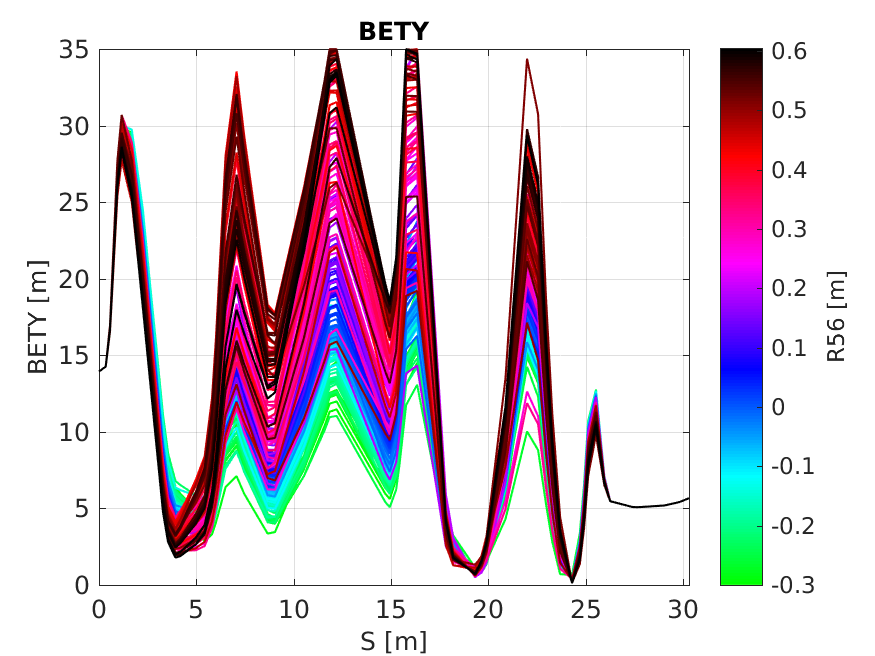
\includegraphics[width=0.8\textwidth]{Figures/propagation/BETY}
  \caption{Vertical beta function in each set of optics for TL1, with the colour scale indicating the \(R_{56}\) value in TL1 for that optics.}
  \label{f:tl1BETY}
\end{figure}

\begin{figure}
  \centering
  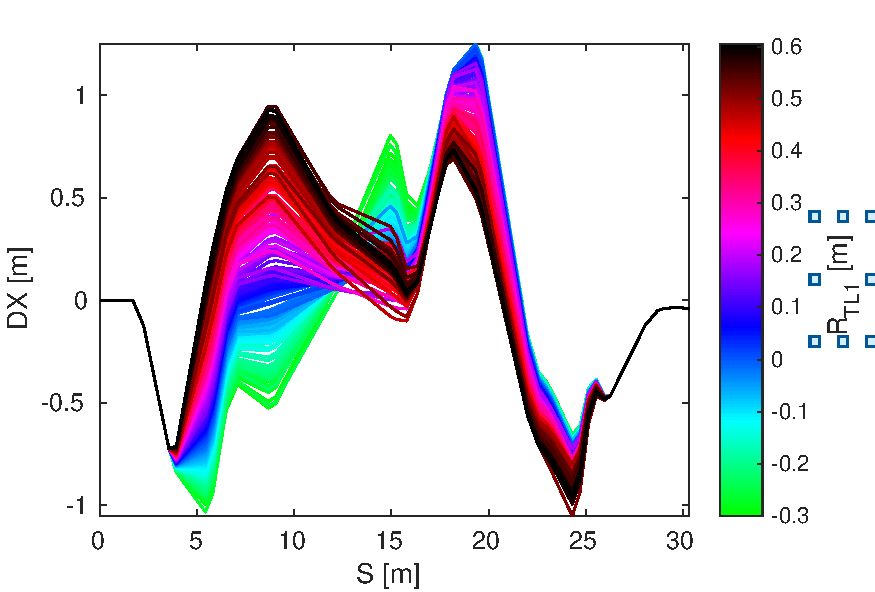
\includegraphics[width=0.8\textwidth]{Figures/propagation/DX}
  \caption{Horizontal dispersion in each set of optics for TL1, with the colour scale indicating the \(R_{56}\) value in TL1 for that optics.}
  \label{f:tl1DX}
\end{figure}

Commissioning of the new TL1 optics in CTF3 was straightforward and in general they can be set with the quadrupole strengths at their nominal matched values without causing issues for the beam quality. At the extremities of the range of optics (close to R56 = -0.1~m and R56 = +0.6~m) some slight beam losses do begin to occur, but this is not a problem for PFF operation where the required R56 is only 0.2~m. However, for each set of optics the magnetic correctors in TL1 may need to be changed to recover the nominal beam orbit, thus taking in to account slight misalignments in elements along the line.

\subsection{Scans of R56 in TL1}
\label{ss:r56Scans}

The sets of matched optics from the previous section can be used to perform scans of the R56 value in TL1 to observe how the downstream phase is affected. Scans of this type must be performed prior to all PFF data taking periods in order to optimise the beam conditions (maximise the upstream-downstream phase correlation) for the correction. More recently scans of R56 in TL1 have been performed whilst varying the beam energy, which produces cleaner results and highlights additional factors that must be taken in to account during the optimisation process, as will be shown in Section~\ref{s:t566}. 

As a starting point the simplest case, where only the TL1 optics is changed during the scan and all other parameters in the machine are left unchanged, is presented in this section. This also highlights some of the difficulties in maintaining beam conditions at CTF3, which is discussed further in Section~\ref{s:t566} and extensively in the context of the PFF correction in Section~\ref{s:longPFF}. Figures~\ref{f:r56Scan_meanPhaseJit}~and~\ref{f:r56Scan_correlation} show one example of an R56 scan performed across the full range of available optics -- from -0.1~m R56 in TL1 to +0.6~m. The R56 is incremented by 2.5~cm between datasets, to give a total of 29 R56 points in the scan, with the whole scan taking approximately one and a half hours to complete. With the knowledge gained from measurements of this type it is no longer necessary to scan the R56 across the full range to determine the ideal value, thus the optimisation of the phase propagation for PFF attempts can now be achieved on much shorter time scales.

\subsubsection{Mean Phase}

Only the mean phase jitters and correlation will be considered here, features along the pulse are discussed in later sections for other scans. Figure~\ref{f:r56Scan_meanPhaseJit} shows the mean phase jitter during the scan both upstream and downstream. Although the noise in the measurement is quite large, the downstream phase jitter is reduced from above 2.5 degrees with zero R56 in TL1, to below 1 degree and close to the level of the upstream phase jitter by adding positive R56 in TL1. The optimal R56 value is approximately 0.175~m, in close agreement with expectations considering the -0.2~m R56 in TL2. The upstream-downstream phase correlation, in Figure~\ref{f:r56Scan_correlation}, is also maximised at this point, from an initial correlation of 20\% with zero R56 to up to 80\%. In terms of the PFF system, increasing the upstream-downstream phase correlation from 20\% to 80\% improves the theoretical correction from a 2\% reduction in downstream phase jitter to a 40\% decrease (Equation~\ref{e:theoretJitOptGain}).

\begin{figure}
  \centering
  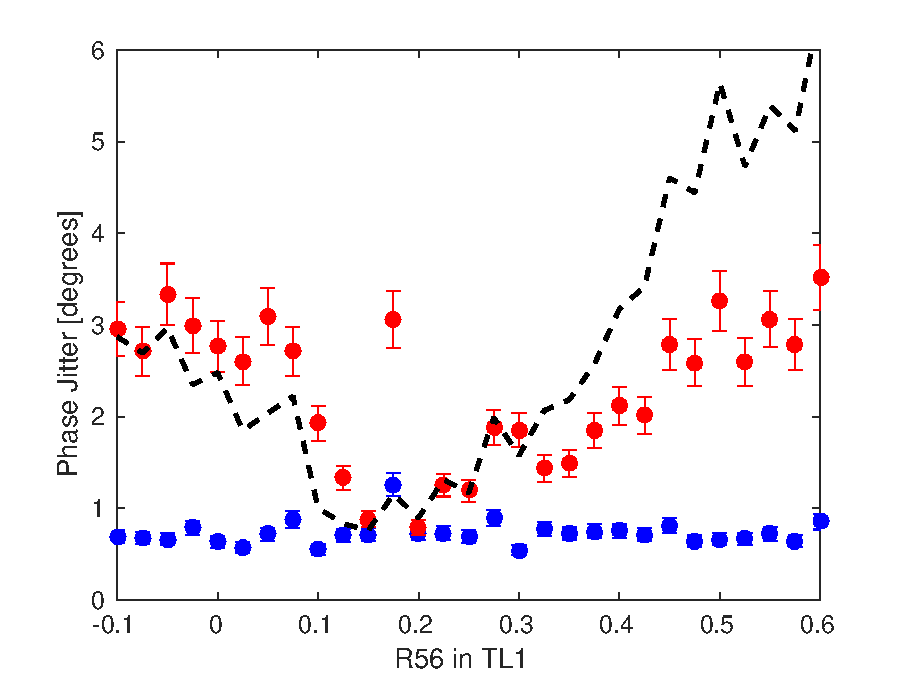
\includegraphics[width=0.8\textwidth]{Figures/propagation/r56Scan_meanPhaseJit}
  \caption{Phase jitter upstream (blue) and downstream (red) during a scan of \(R_{56}\) in TL1. The dashed line shows a simulation of the expected downstream phase jitter given the beam conditions in each dataset.}
  \label{f:r56Scan_meanPhaseJit}
\end{figure}

\begin{figure}
  \centering
  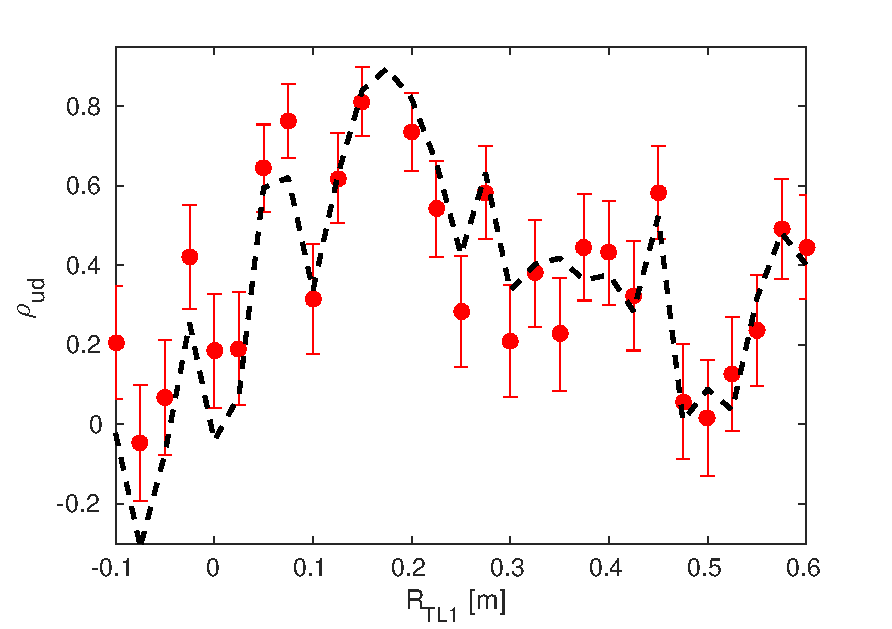
\includegraphics[width=0.8\textwidth]{Figures/propagation/r56Scan_correlation}
  \caption{Upstream-downstream phase correlation (red) during a scan of \(R_{56}\) in TL1. The dashed line shows a simulation of the expected downstream phase jitter given the beam conditions in each dataset.}
  \label{f:r56Scan_correlation}
\end{figure}

As the upstream phase monitors are prior to TL1, changing the TL1 optics has no effect on the upstream phase jitter. All differences in the upstream phase jitter between datasets are caused by drifts in the CTF3 injector, typically changes in either klystron phases or beam current. Although the overall stability of the upstream phase jitter during this scan is good, it does vary between 0.5~degrees and 1.2~degrees. In addition to the upstream phase there are also differences in the relative energy jitter and upstream phase-energy correlation during the scan, as seen in Figure~\ref{f:r56Scan_upstreamParams}. The relative beam energy jitter varies between \(0.4\times10^{-3}\) and \(1.0\times10^{-3}\) and the upstream phase-energy correlation between -0.5 and +0.5. All these parameters influence the downstream phase, as per the equations in Section~\ref{ss:r56Equations}.

The differences in the upstream phase and energy conditions between datasets partially explains the apparent spread of the data points away from the expected clean distribution. The black ``simulation'' lines in Figures~\ref{f:r56Scan_meanPhaseJit}~and~\ref{f:r56Scan_correlation} represent the expected downstream phase jitter and upstream-downstream phase correlation at each point in the scan given the upstream phase jitter, relative energy jitter and upstream phase-energy correlation at that time (using Equations~\ref{e:r56JitEq}~and~\ref{e:r56CorrDefFinal}). The correlation simulation in Figure~\ref{f:r56Scan_correlation} has been scaled so that the peak value is in agreement with the data, at 0.8. The majority of the data points follow the scaled simulated distribution, with several remaining outliers. For the downstream phase jitter (which uses the simulated result directly with no scaling) the agreement with the simulation is generally good for R56 values below 0.3~m. However, above 0.3~m the actual phase jitter seen in the scan is smaller than the simulation. One possible explanation for this are the changes in downstream beam current between datasets, which varies by a factor 3 during the scan (bottom plot in Figure~\ref{f:r56Scan_upstreamParams}). Small beam losses between measurements may change the phase jitter in a way that is not characterised by the R56. Possible other sources are discussed in Sections~\ref{s:t566}~and~\ref{s:otherJitterSources}.

\begin{figure}
  \centering
  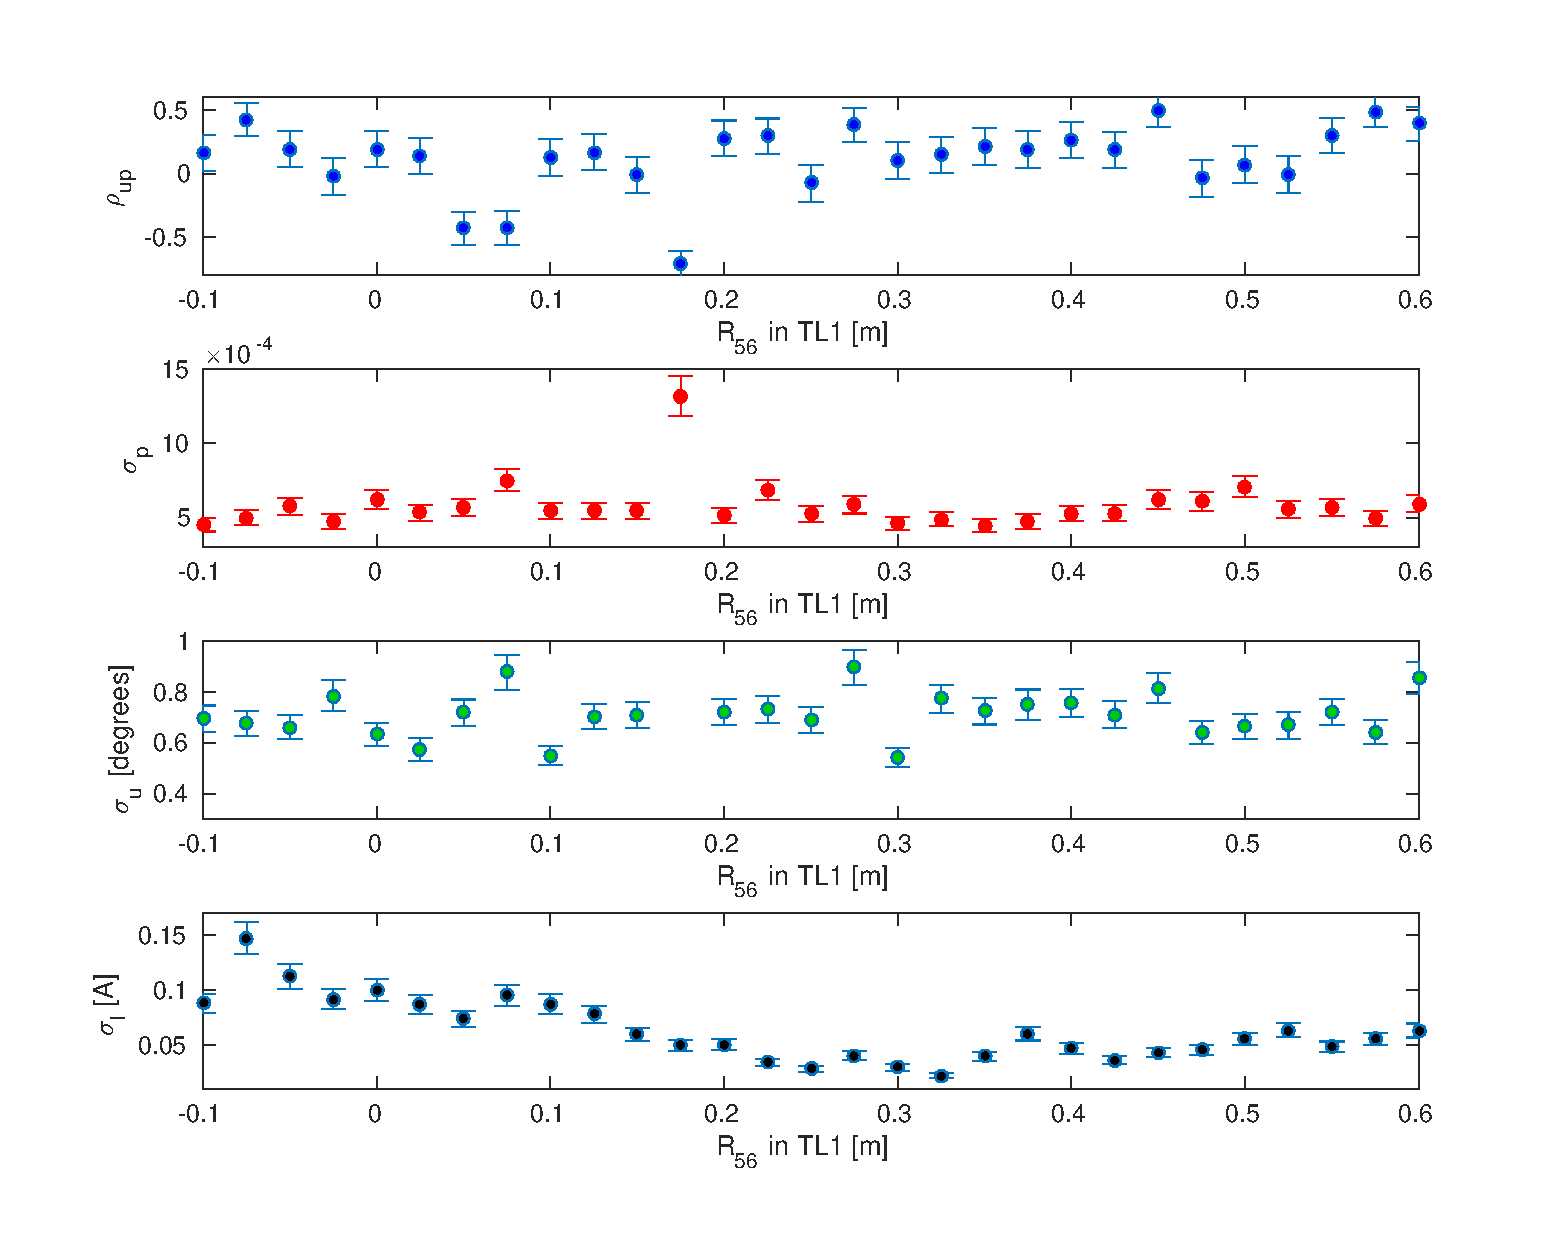
\includegraphics[width=\textwidth]{Figures/propagation/r56Scan_upstreamParams}
  \caption{Upstream and downstream beam conditions during the R56 scan. From top to bottom: upstream phase-energy correlation (blue), relative energy jitter (red), upstream phase jitter (green) and beam current jitter (black).}
  \label{f:r56Scan_upstreamParams}
\end{figure}

\subsubsection{Results from Other Scans}

\begin{figure}
  \centering
  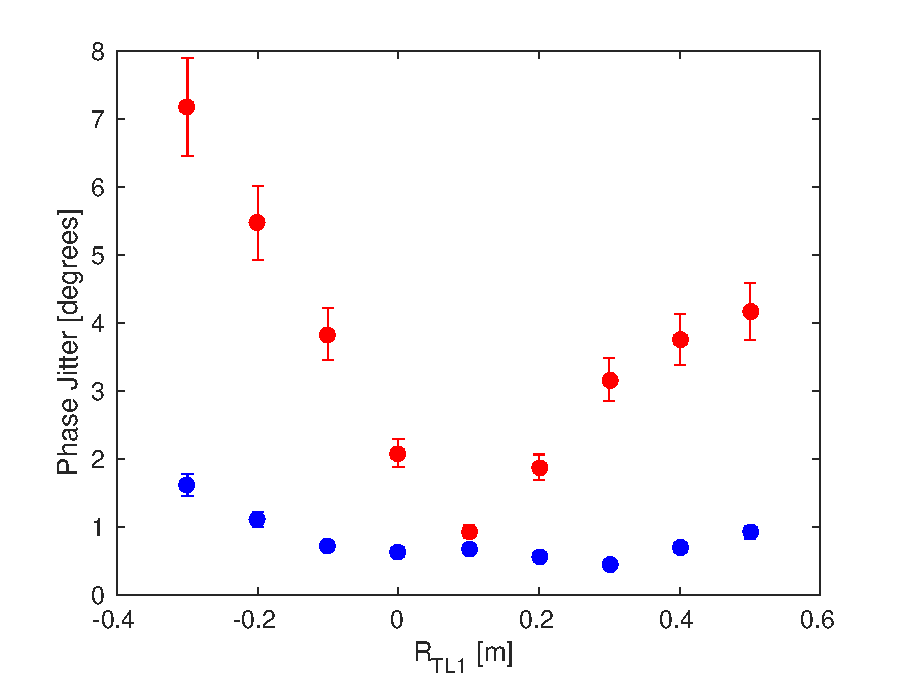
\includegraphics[width=0.8\textwidth]{Figures/propagation/r56Scan2_meanJitter}
  \caption{Upstream (blue) and downstream (red) phase jitter during an \(R_{56}\) scan in TL1 showing an optimal set point of around \(R_{56}=0.1\)~m.}
  \label{f:r56Scan2_meanJitter}
  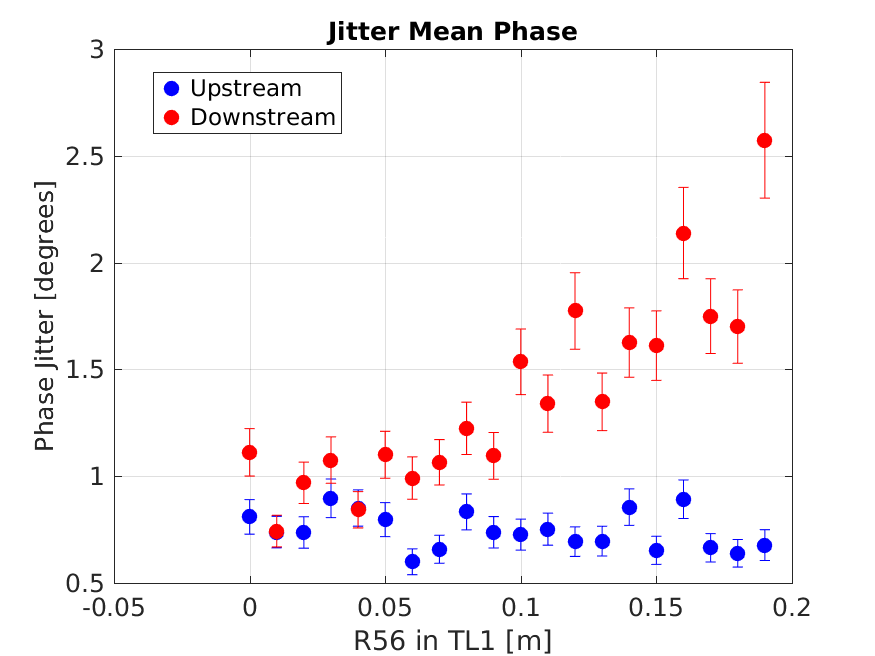
\includegraphics[width=0.8\textwidth]{Figures/propagation/r56Scan3_meanJitter}
  \caption{Upstream (blue) and downstream (red) phase jitter during an \(R_{56}\) scan in TL1 showing an optimal set point of \(R_{56}<0.05\)~m.}
  \label{f:r56Scan3_meanJitter}
\end{figure}


Figures~\ref{f:r56Scan2_meanJitter}~and~\ref{f:r56Scan3_meanJitter} show the results of two further scans of R56 in TL1, both taken a few days after the scan previously shown. For both scans the mean downstream phase jitter can again be decreased to the level of the upstream phase jitter by varying the R56 in TL1, and the upstream-downstream correlation increased to 80\%. However, the optimal optics to use is different for each scan --- the scan in Figure~\ref{f:r56Scan2_meanJitter} has an optimal R56 value of around 0.1~m whereas for the scan in Figure~\ref{f:r56Scan3_meanJitter} the optimal value quite close to zero, around 0.04~m. Both values are also different to the scan previously shown, which had an optimal R56 setting of 0.175~m.

With R56 alone and the model of the phase propagation used to derive the equations in Section~\ref{ss:r56Equations} there is no mechanism for the optimal R56 value to vary with time. The best conditions for the phase propagation should always be provided with zero residual R56 between the upstream and downstream phase monitors. As the optics in all beam lines between the upstream and downstream phase monitors (apart from TL1) were unchanged between each scan, the optimal R56 value in TL1 should also be the same for each scan in this model. The most likely explanation is a sensitivity to higher order energy dependencies.

\newsection{t566}{Higher Order Energy Dependencies}

In the same way the first oder optics dependencies are described by the \(6 \times 6\) R-matrix, the second order effects are described using a three dimensional \(6 \times 6 \times 6\) T-matrix. \(R_{56}\) is the relevant first order transfer matrix coefficient for the energy related effects on the phase propagation, as already discussed, and it then follows that the relevant T-matrix coefficient for second order energy dependencies is \(T_{566}\). By including the second order term the dependence of the downstream phase on the energy from Equation~\ref{e:r56PhasEq} becomes:
\begin{equation}
\phi_d = \phi_u + R_{56}\left(\frac{\Delta p}{p}\right) + T_{566}\left(\frac{\Delta p}{p}\right)^2
\label{e:t566}
\end{equation}

\(T_{566}\) introduces another source of energy dependent phase jitter which is independent from the first order \(R_{56}\) value. The ideal case for the phase propagation would be to have both zero \(R_{56}\) and zero \(T_{566}\) between the upstream and downstream phase monitors. However, constraints are not placed on the \(T_{566}\) in the optics at CTF3 and it is therefore typically non-zero. It may be possible to create optics with zero, or at least reduced, \(T_{566}\) for the TL1 and TL2 lines at CTF3 in the future but this has not yet been pursued, thus it will be treated as a fixed property of the optics here. In this case an expression for the \(R_{56}\) value that minimises the downstream phase-energy dependence can be derived:
\begin{equation}
R_{56} = -2T_{566} \left(\frac{\Delta p}{p}\right)
\label{e:r56t566dep}
\end{equation}
This is obtained by zeroing the partial differential of Equation~\ref{e:t566} with respect to \(\Delta p/p\).

The above dependence of the \(R_{56}\) value on the beam energy offset has many consequences. Firstly, it provides a mechanism by which the apparent optimal \(R_{56}\) value in TL1 can vary with time (and be non-zero), as was seen comparing the results of different \(R_{56}\) scans in the previous section. CTF3 does experience drifts in beam energy (Section~\ref{ss:energyVariations}), creating small offsets between the actual beam energy and the energy that the optics has been set for (i.e. the strength of bending and focusing elements in the accelerator). In other words, it is possible for the mean of \(\Delta p / p\) to be non-zero. The optimal \(R_{56}\) value to use in TL1 is therefore expected to drift with the beam energy when higher order phase-energy dependencies are included.

Secondly, energy variations along the beam pulse and jitter in the beam energy mean that the phase propagation cannot be perfectly optimised by varying the \(R_{56}\) alone. Due to the energy dependence in Equation~\ref{e:r56t566dep}, any energy variations along the pulse cause the optimal \(R_{56}\) value to set in TL1 to also vary along the beam pulse. There are static variations in the mean energy along the pulse (e.g. as seen in Section~\ref{ss:energyVariations}) at CTF3, so this means the phase propagation can never be completely optimised along the full pulse length when \(T_{566}\) is non-zero. 

\subsection{Simulated Effect of \(T_{566}\) on the Downstream Phase}
\label{ss:t566Sim}

When only the first order effect of \(R_{56}\) is considered the dependence of the downstream phase on the energy is linear, with the gradient depending on the residual \(R_{56}\) value between the upstream and downstream phase monitors. The downstream phase versus beam energy offset with only first order \(R_{56}\) term included is shown in Figure~\ref{f:phaseVsEn_r56Only} for each set of TL1 optics, demonstrating this effect. The optimal \(R_{56}\) value of \(+0.2\)~m in TL1 minimises the phase-energy dependence for all energy offsets.

\begin{figure}
  \centering
  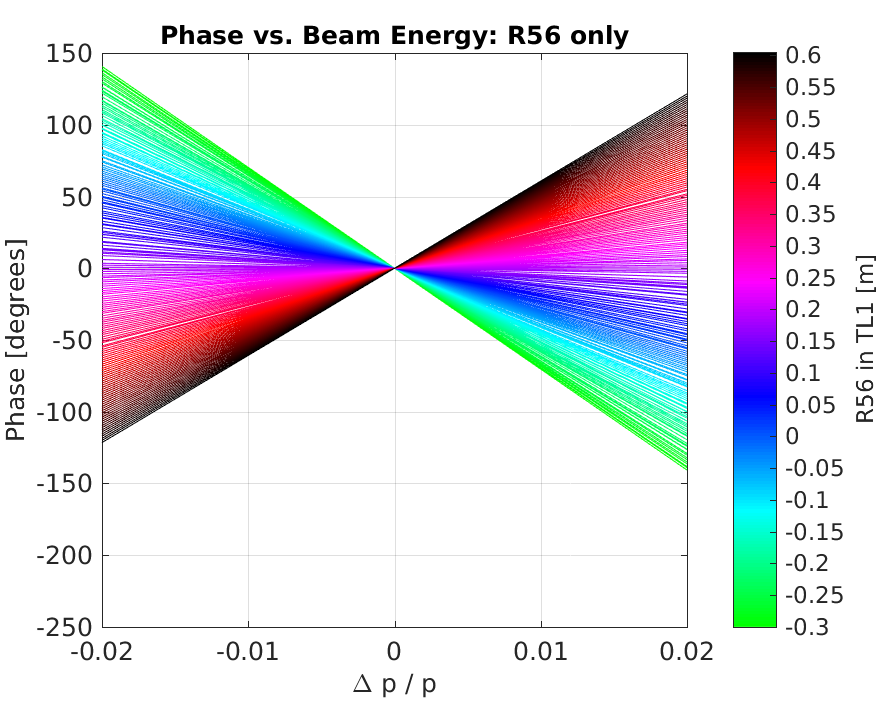
\includegraphics[width=0.8\textwidth]{Figures/propagation/phaseVsEn_r56Only}
  \caption{Dependence of the downstream phase on the relative energy offset for all sets of TL1 optics when only \(R_{56}\) is considered.}
  \label{f:phaseVsEn_r56Only}  
  \centering
  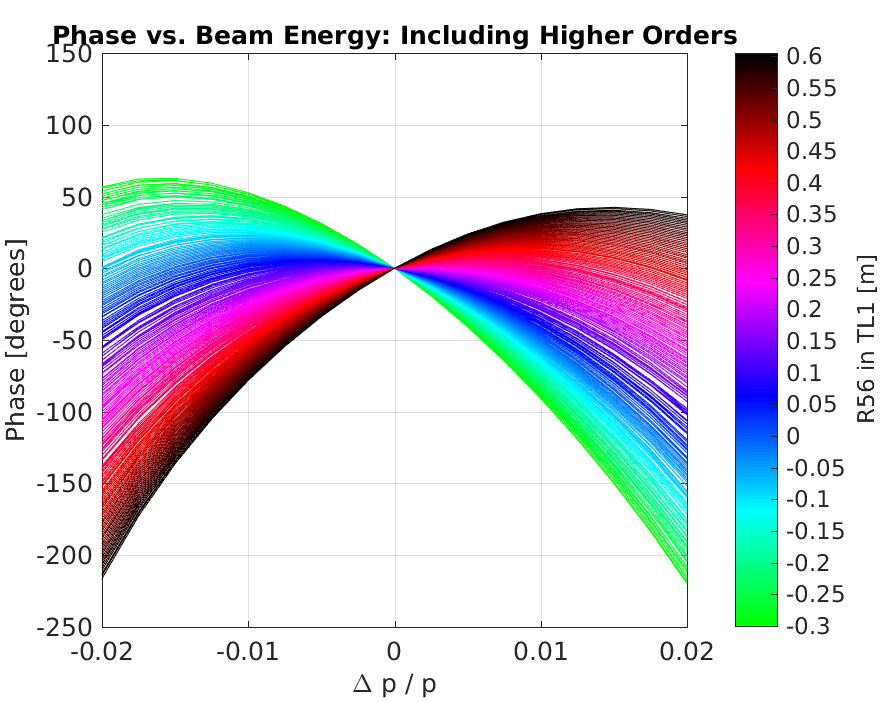
\includegraphics[width=0.8\textwidth]{Figures/propagation/phaseVsEn_t566}
  \caption{Dependence of the downstream phase on the relative energy offset for all sets of TL1 optics including higher order effects.}
  \label{f:phaseVsEn_t566}
\end{figure}

By running MADX with varying energy offsets set in the initial conditions the expected effect of the higher order energy dependencies on the downstream phase can be seen. This is shown in Figure~\ref{f:phaseVsEn_t566}, and the impact of the higher orders is immediately clear. The optimal \(R_{56}\) to use in TL1, where the phase has the minimal dependence on the energy (at the peaks of the phase-energy curves in the figure), now depends on the energy offset. Figure~\ref{f:optR56vsEnergy} shows that the dependence of the optimal \(R_{56}\) value on the relative energy offset is linear, as expected from Equation~\ref{e:r56t566dep}. The plotted \(R_{56}\) value does not exceed \(+0.6\)~m or go below \(-0.3\)~m as only the available sets of optics for TL1 are considered, which are restricted to this range. This also creates small non-linearities in the central region of the plot, although there is also a contribution from effects above second order. 


\begin{figure}
  \centering
  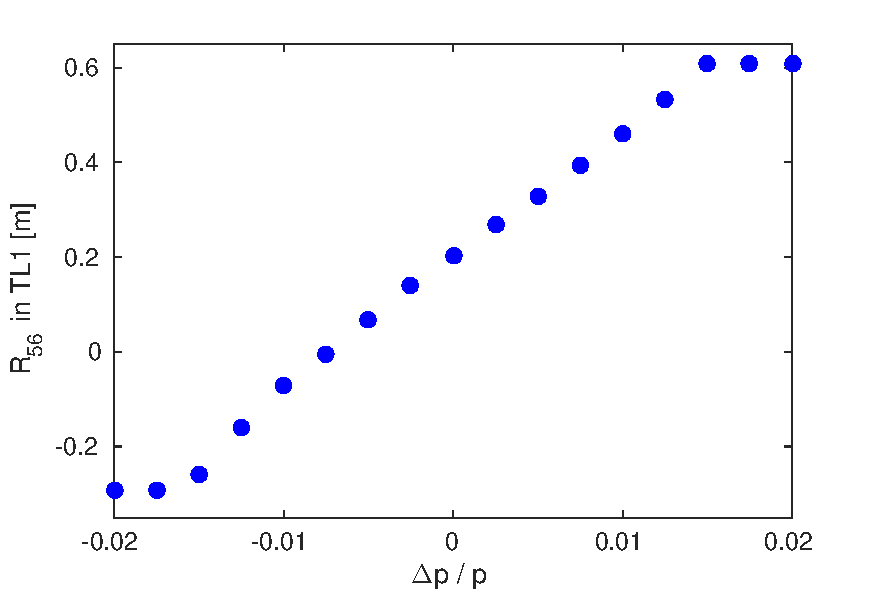
\includegraphics[width=0.8\textwidth]{Figures/propagation/optR56vsEnergy}
  \caption{Dependence of the optimal optics to use in TL1 on the relative energy offset.}
  \label{f:optR56vsEnergy}
\end{figure}

MADX does not output the optics \(T_{566}\) coefficient directly but it can be approximated using a quadratic fit to the downstream phase vs. energy curves seen in Figure~\ref{f:phaseVsEn_t566}. The fit coefficients then give the \(T_{566}\) and \(R_{56}\) values, as per Equation~\ref{e:t566}. An example of this is shown in Figure~\ref{f:madxT566Fit} for the nominal \(R_{56}=0\) optics in TL1. Again, as the results from MADX also includes effects above second order there is a slight discrepancy between the quadratic fit and the MADX output. However, including up to the second order energy dependence is enough to characterise the true behaviour and the slight modifications induced by higher orders are beyond the scope of the discussion here.

\begin{figure}
  \centering
  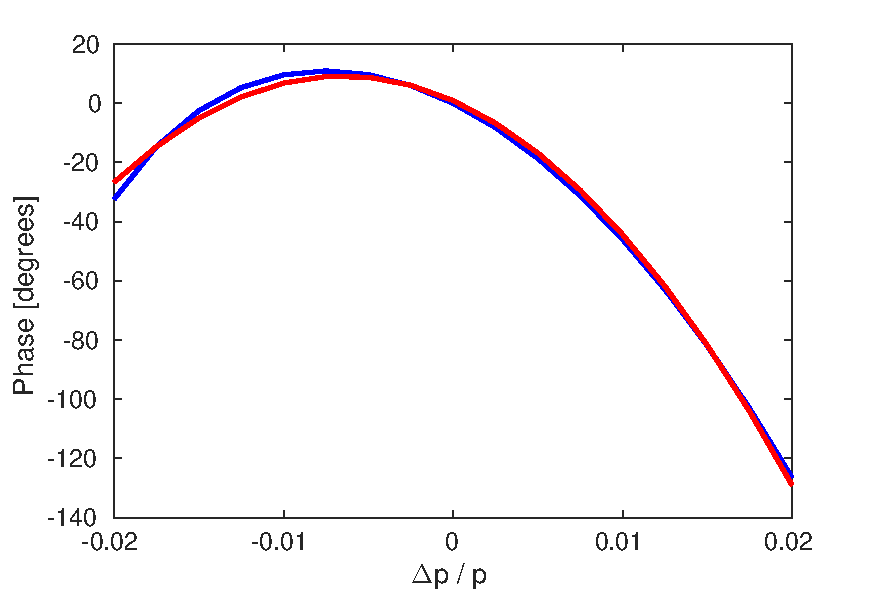
\includegraphics[width=0.8\textwidth]{Figures/propagation/madxT566Fit}
  \caption{Quadratic fit (red) to the simulated downstream phase from MADX for different energy offsets (blue).}
  \label{f:madxT566Fit}
\end{figure}

Figure~\ref{f:t566TotVsr56TL1} then shows the fitted \(T_{566}\) coefficient for all the sets of matched optics in TL1. The changes in \(T_{566}\) across the range of TL1 optics are much smaller than the (intentional) differences in \(R_{56}\), varying between -13.1~m and -15.4~m. Optics around the usually optimal \(R_{56}\) value of 0.2~m in TL1  are close to where the second order effects are minimal, with \(T_{566}\) values around -13.4~m. The \(T_{566}\) coefficients are approximately two orders of magnitude larger than the \(R_{56}\) but as \(\left(\Delta p / p\right)^2 << \left(\Delta p / p\right) << 1\) the effect on the phase is smaller than for non-optimised \(R_{56}\). For example, for a typical relative energy offset of \(1 \times 10^{-3}\) a residual \(R_{56}\) of 0.2~m between the upstrem and downstream phase monitors leads to a phase shift of more than one degree. For the same energy offset the phase shift resulting from the second order \(T_{566}\) term is approximately 0.1 degrees. However, the key point for the phase propagation is that the first order dependence can be removed by zeroing \(R_{56}\) between the upstream and downstream phase monitors, whereas for all the available sets of optics the second order contribution will remain at roughly the same magnitude.

\begin{figure}
  \centering
  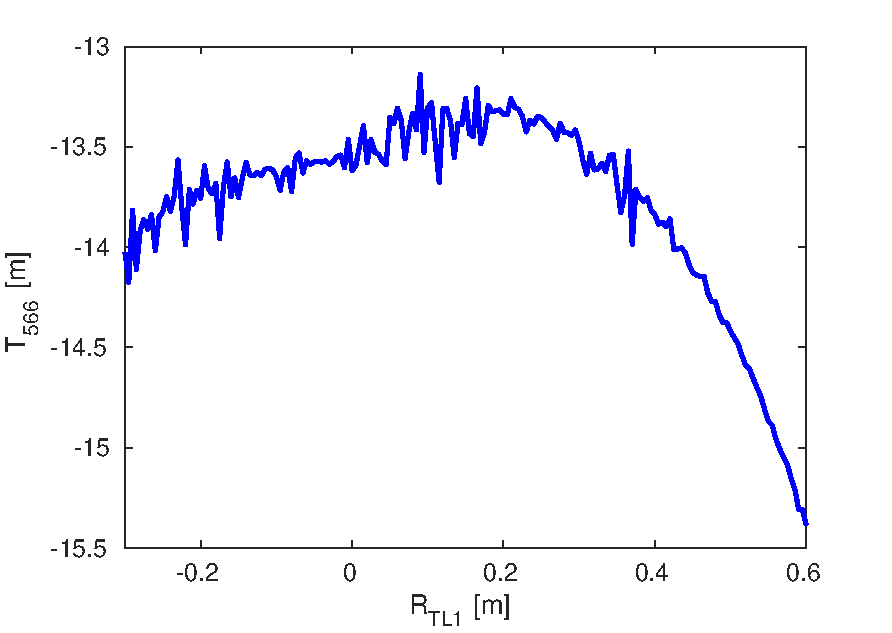
\includegraphics[width=0.8\textwidth]{Figures/propagation/t566TotVsr56TL1}
  \caption{\(T_{566}\) coefficient between the upstream and downstream phase monitors for all sets of TL1 optics.}
  \label{f:t566TotVsr56TL1}
\end{figure}

To determine the consequences of the \(T_{566}\) for the PFF system the effect it has on the upstream-downstream phase correlation and downstream phase jitter must be calculated. This was done analytically using the equations in in Section~\ref{ss:r56Equations} for the first order \(R_{56}\), but for the second order terms a simple Monte Carlo simulation approach has been used. Correlated random distributions are created in MatLab to match the typical CTF3 upstream phase and energy conditions --- namely \(\sigma_p = 0.001\), \(\sigma_u = 0.8^\circ\) and \(\rho_{up} = 0.2\). The simulated downstream phase for each set of TL1 optics is then calculated using Equation~\ref{e:t566} and the known \(R_{56}\) and \(T_{566}\) values. The jitter of this simulated downstream phase and its correlation with the initial upstream phase distribution give the values shown in the following figures.

The solid lines in Figure~\ref{f:jitVsR56_t566} show the downstream phase jitter versus the residual \(R_{56}\) between the upstream and downstream phase monitors in the case where only the first oder \(R_{56}\) term is included (red) and when both the \(R_{56}\) and the second order \(T_{566}\) are included (blue). The effect of including \(T_{566}\) is very small, with the downstream phase jitter only increasing from \(0.80^\circ\) to \(0.85^\circ\) degrees at the optimal residual \(R_{56}\) of zero. The effect of including \(T_{566}\) on the upstream-downstream phase correlation is much more significant for the PFF correction. The maximum achievable correlation (excluding the effects of the phase monitor resolution) is reduced from \(\rho_{ud} = 1\) with only the first order term to \(\rho_{ud} = 0.95\) when \(T_{566}\) is included. This is shown in Figure~\ref{f:corrVsR56_t566}.  This increases the achievable corrected downstream phase jitter with the PFF systen from zero to \(0.27^\circ\) (again excluding the phase monitor resolution). 

\begin{figure}
  \centering
  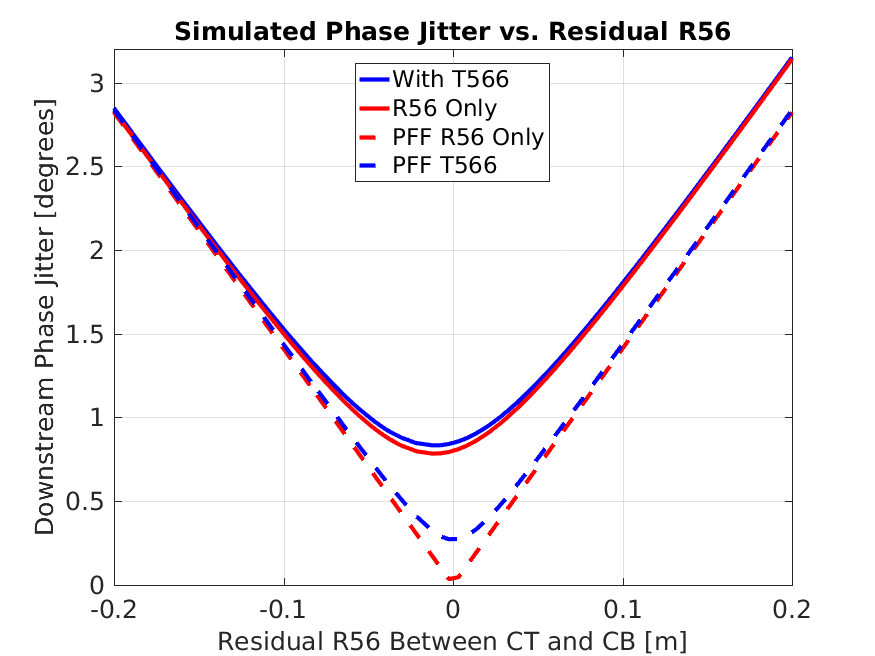
\includegraphics[width=0.8\textwidth]{Figures/propagation/jitVsR56_t566}
  \caption{Downstream phase jitter vs. \(R_{56}\) between the upstream and downstream phase monitors. Blue lines include the effects of both \(R_{56}\) and \(T_{566}\), whereas red lines include only the first order \(R_{56}\) term. Solid lines show the initial downstream jitter, and dashed lines the achievable corrected downstream phase jitter. Beam conditions of \(\sigma_u = 0.8^\circ\), \(\rho_{up}=0.2\) and \(\sigma_p = 1 \times 10^{-3}\) are used for the simulation.}
  \label{f:jitVsR56_t566}
  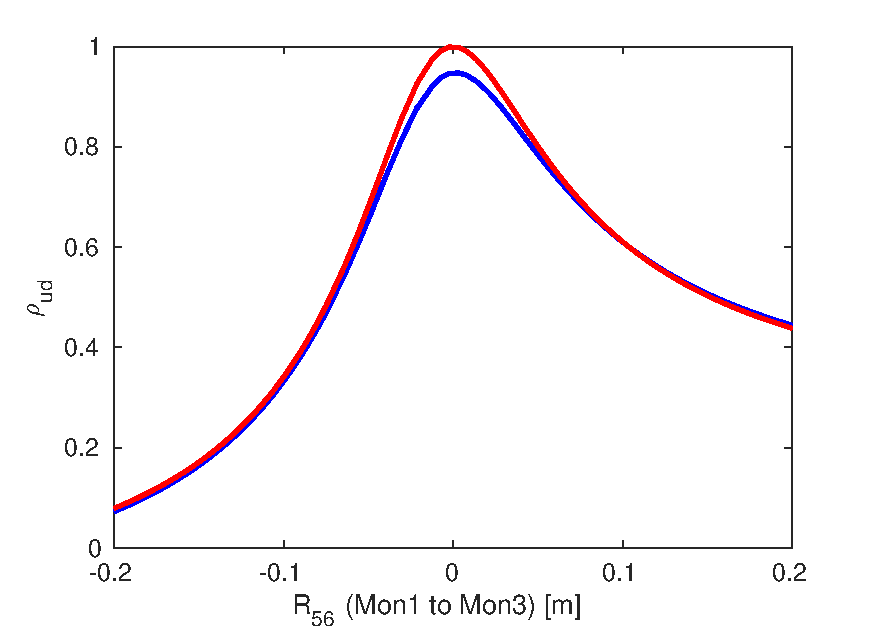
\includegraphics[width=0.8\textwidth]{Figures/propagation/corrVsR56_t566}
  \caption{Upstream-downstream phase correlation vs. \(R_{56}\) between the upstream and downstream phase monitors. The blue line includes the effects of both \(R_{56}\) and \(T_{566}\), whereas the red line includes only the first order \(R_{56}\) term.  Beam conditions of \(\sigma_u = 0.8^\circ\), \(\rho_{up}=0.2\) and \(\sigma_p = 1 \times 10^{-3}\) are used for the simulation.}
  \label{f:corrVsR56_t566}
\end{figure}

With the initial conditions and optics used here it would therefore be impossible to achieve \(0.2^\circ\) phase stability at CTF3. However, the relative energy jitter of \(1\times10^{-3}\) is in fact somewhat pessimistic for the conditions that can be achieved at CTF3, at least on short time scales. Figure~\ref{f:maxCorrWithT566} shows how the maximum achievable upstream-downstream phase correlation varies with the relative energy jitter. An upstream-downstream phase correlation of 97\% is required to make achieving \(0.2^\circ\) downstream phase jitter at CTF3 possible. This can be achieved with a relative energy jitter of \(0.85\times10^{-3}\) if the \(R_{56}\) is perfectly optimised. In good conditions, especially with recent developments (Section~\ref{ss:t566Mitigation}), the CTF3 energy jitter can be reduced to around \(0.5\times10^{-3}\), in which case correlations up to \(99.6\%\) are theoretically achievable. It should therefore still be possible to achieve the necessary conditions for the PFF system at CTF3 even after taking in to account \(T_{566}\).

\begin{figure}
  \centering
  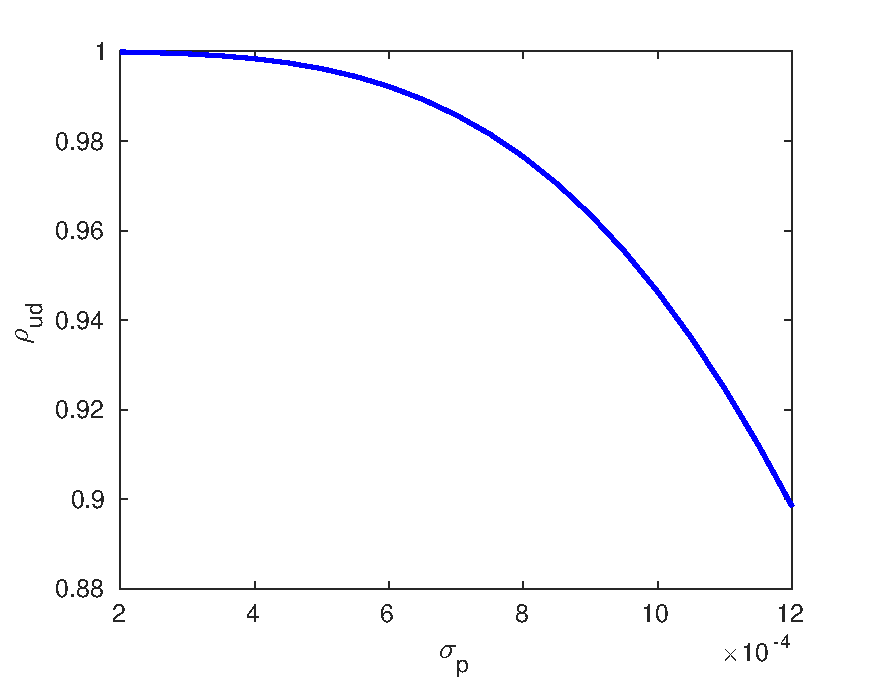
\includegraphics[width=0.8\textwidth]{Figures/propagation/maxCorrWithT566}
  \caption{Best possible upstream-downstream phase correlation vs. beam energy jitter both with (blue) and without (red) including the second order \(T_{566}\) term.}
  \label{f:maxCorrWithT566}
  \centering
  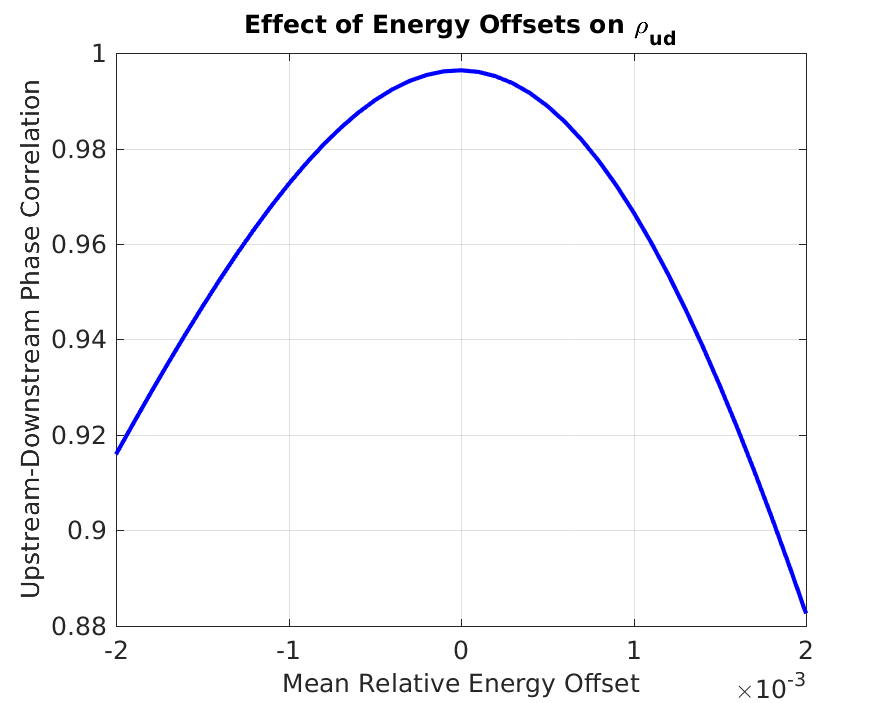
\includegraphics[width=0.8\textwidth]{Figures/propagation/corrVsEnergyOffset}
  \caption{Upstream-downstream phase correlation vs. relative beam energy offset including the second order effects of \(T_{566}\).}
  \label{f:corrVsEnergyOffset}
\end{figure}

One final consequence of the non-zero \(T_{566}\) between the upstream and downstream phase monitors is the effect of energy variations along the pulse, or equivalently cases where the mean value of \(\Delta p/p\) is non-zero. All previous calculations have assumed the energy jitter to be about a mean \(\Delta p / p\) of zero, but this can not be true for all points along the CTF3 pulse due to the variations in mean beam energy along the pulse seen in Section~\ref{ss:energyVariations}. The effect of mean energy offsets on the upstream-downstream phase correlation is shown in Figure~\ref{f:corrVsEnergyOffset}, in this case assuming a relative energy jitter of \(0.5\times10^{-3}\) about the offset mean value and zero \(R_{56}\). Typically the energy variation along the CTF3 pulse is at the \(\pm2\times10^{-3}\) level, and this by itself can cause the correlation to drop below 90\%. As a result the achievable corrected downstream phase jitter with the PFF system will also vary along the pulse. Without reducing either the energy variations along the pulse, or changing the optics to decrease the magnitude of \(T_{566}\), it is unlikely that \(0.2^\circ\) sample-by-sample jitter along the pulse can be achieved for more than very short portions of the pulse where the energy is optimal. Reducing energy variations along the pulse to below \(\pm1 \times10^{-3}\) would allow correlations above 96\% to be achieved across the full pulse length, increasing the feasibility of hitting the \(0.2^\circ\) target. New feedbacks have been developed at CTF3 to try to achieve this (Section~\ref{ss:t566Mitigation}).



\subsection{R56 Scans whilst Varying Beam Energy}
\label{ss:r56ScanWithEnergy}

By intentionally varying the CTF3 beam energy to artificially increase the energy jitter during an \(R_{56}\) scan the energy dependent effects in both the upstream and the downstream phase are amplified. This has the benefit of increasing the visibility of the higher order effects, but it also improves the results of the scan in general by reducing the sensitivity to other small drifts in beam conditions. In this section the results of an \(R_{56}\) scan in which the \(R_{56}\) value in TL1 was varied between -0.1~m and +0.3~m whilst the beam energy was varied by approximately 1\% peak-to-peak are discussed. The resulting relative energy jitter of \(3\times10^{-3}\) in these conditions is 3--5 times larger than the relative energy jitter in nominal conditions. Direct observations of the effect of higher order energy dependencies during the scan will be presented first, before discussing the overall results of the scan to expand upon the conclusions from the \(R_{56}\) scans shown in previous sections.

\subsubsection{Energy Dependence}

Figure~\ref{f:R56ScanGunWiggle_PhaseVsEnergy} shows the dependence of the mean downstream phase on the beam energy for three of the \(R_{56}\) values set in TL1 during the scan -- the lowest value of \(-0.1\)~m, the maximum value of \(0.3\)~m and a mid-range value of \(0.075\)~m, which gives the lowest downstream phase jitter during the scan as seen later in this section. This plot mimics the simulated result from MADX in Figure~\ref{f:phaseVsEn_t566}. With the increased energy jitter the non-linear dependence of the downstream phase on the energy is clear. The first order effect means changing the \(R_{56}\) value changes the gradient of the phase-energy dependence about the central energy. The effect of \(T_{566}\) means there is an energy dependent \(R_{56}\) value that minimises the gradient. For example, with an \(R_{56}\) of -0.1~m set in TL1 energy offsets around \(-5\times10^{-3}\) give the minimum energy dependence.

\begin{figure}
  \centering
  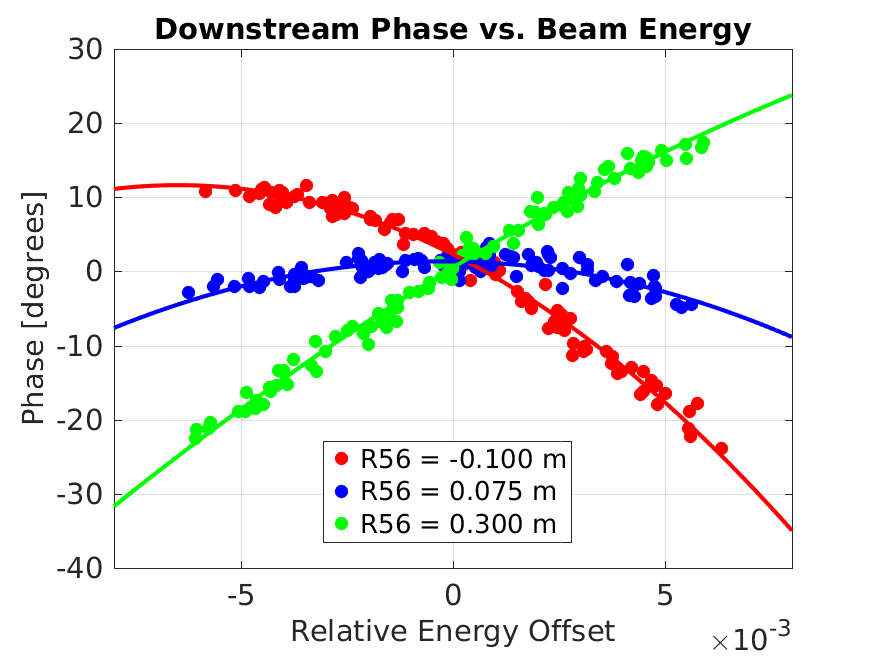
\includegraphics[width=0.8\textwidth]{Figures/propagation/R56ScanGunWiggle_PhaseVsEnergy}
  \caption{Measured downstream phase vs. beam energy for three different set of \(R_{56}\) optics in TL1: \(R_{56}=-0.100\)~m (red), \(R_{56}=0.075\)~m (blue), and \(R_{56}=0.300\)~m (green). Lines show quadratic fits to the data for each set of optics.}
  \label{f:R56ScanGunWiggle_PhaseVsEnergy}
\end{figure}

\begin{figure}
  \centering
  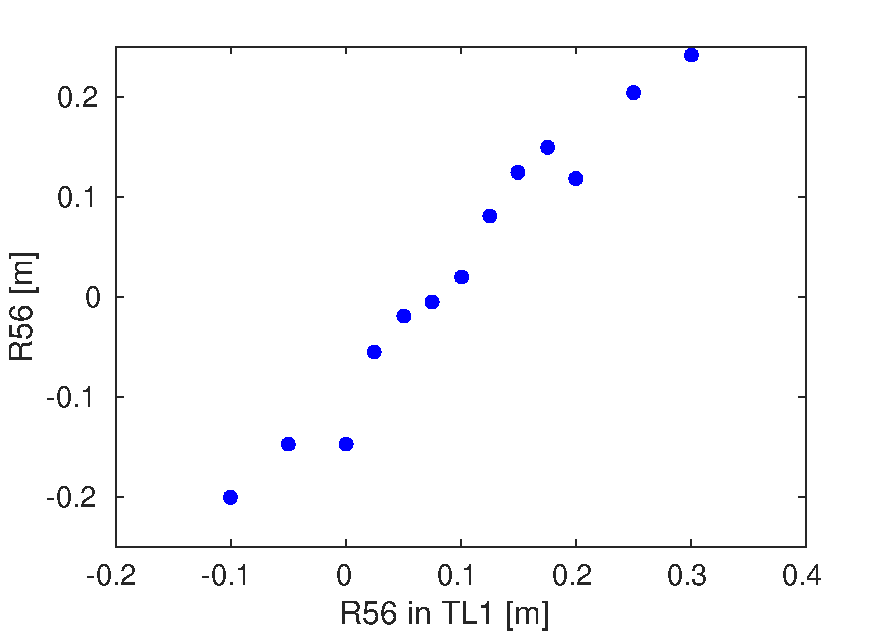
\includegraphics[width=0.8\textwidth]{Figures/propagation/R56ScanGunWiggle_R56Fit}
  \caption{Fitted total \(R_{56}\) value between the upstream and downstream phase monitors for each \(R_{56}\) value applied in TL1 during the scan.}
  \label{f:R56ScanGunWiggle_R56Fit}
  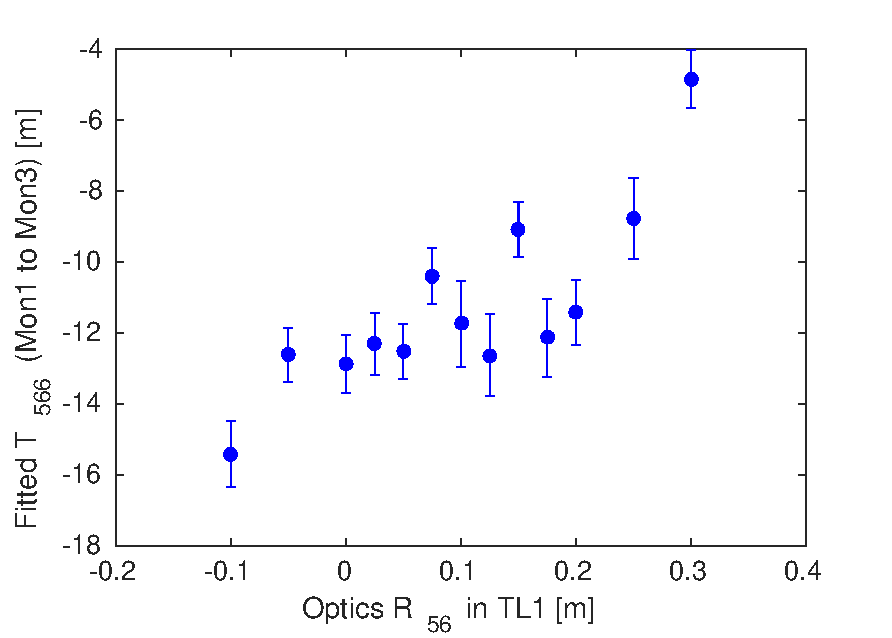
\includegraphics[width=0.8\textwidth]{Figures/propagation/R56ScanGunWiggle_T566Fit}
  \caption{Fitted \(T_{566}\) value between the upstream and downstream phase monitors for each set of \(R_{56}\) optics applied in TL1 during the scan.}
  \label{f:R56ScanGunWiggle_T566Fit}
\end{figure}

The coefficients of a quadratic fit to the curves in Figure~\ref{f:R56ScanGunWiggle_PhaseVsEnergy} (plus their equivalents for other points in the scan) give estimates for the residual \(R_{56}\) and \(T_{566}\) values between the upstream and downstream phase monitors. The results of doing this are shown in Figure~\ref{f:R56ScanGunWiggle_R56Fit} for the fitted \(R_{56}\) values, and Figure~\ref{f:R56ScanGunWiggle_T566Fit} for the fitted \(T_{566}\) values. 

The fit \(R_{56}\) values roughly follow a linear dependence on the set \(R_{56}\) optics in TL1, as expected. With an \(R_{56}\) value of -0.2~m in TL2, varying the \(R_{56}\) between -0.1 and +0.3~m in TL1 would be expected to give a total residual \(R_{56}\) of between -0.3~m and +0.1~m. The fitted range is between -0.20~m and +0.25~m, so is +0.1~m offset compared to expectations. The fitted \(R_{56}\) values depend on the absolute mean energy offset, which is not easily verifiable from the BPM measurement measurement alone. Offsetting the mean relative energy offset from zero to \(2\times10^{-3}\) would bring the fitted \(R_{56}\) values close to the expected range.

For \(R_{56}\) values in TL1 up to 0.2~m the fitted \(T_{566}\) values in TL1 in Figure~\ref{f:R56ScanGunWiggle_T566Fit} are close to the simulated values typically around -13.5~m in Figure~\ref{f:madxT566Fit}. For the points above 0.2~m \(R_{56}\) in TL1 in the scan, the fitted \(T_{566}\) value is smaller than expected. However, the measured first and second order energy dependent effects are overall in very good agreement with expectations given the constraints of measurement and accuracy of the MADX model.


\subsubsection{Mean Phase}

Figure~\ref{f:R56ScanGunWiggle_PhaseJitter} shows the mean phase jitter during this \(R_{56}\) scan both upstream and downstream. Simulations of the expected phase jitter given the beam conditions and optics are also shown, both for the case where only \(R_{56}\) is considered and when both \(R_{56}\) and \(T_{566}\) are taken in to account. Varying the beam energy during the scan has the effect of increasing the upstream phase jitter from its typical level of 0.8 degrees to 2.0 degrees. The correlation between the upstream phase and the beam energy is also increased from 20\% in normal conditions to above 90\% whilst varying the beam energy. An example of this is shown in Figure~\ref{f:R56ScanGunWiggle_UpEnCorr} for the dataset at \(R_{56}=-0.1\)~m in TL1. The likely source of the upstream phase-energy dependence is the energy variation leading to differences in beam orbit through the stretching chicane in the CTF3 linac (see Figure~\ref{f:ctfLayout}).

The downstream phase jitter is reduced to close to the level of the upstream phase jitter for \(R_{56}\) values between 0.5~m and 0.1~m in TL1.  Now knowing that the \(T_{566}\) can cause a dependence between the optimal \(R_{56}\) value in TL1 and the beam energy it is not completely unexpected that the lowest downstream phase jitter is not at the 0.2~m expected due to the optics in TL2. An mean relative energy offset of \(-2\times10^-3\) can lead to the minimum jitter being shifted to 0.075~m as seen in the scan. This offset has been used to create the simulated ``\(T_{566}\) Sim'' lines  in Figures~\ref{f:R56ScanGunWiggle_PhaseJitter}~and~\ref{f:R56ScanGunWiggle_Correl}. The simulation including this energy offset and the effects of \(T_{566}\) follows the actual downstream phase jitter during the scan much more closely than the simulation including only \(R_{56}\). There are still differences between the data and the \(T_{566}\) simulation, in particular in the range between \(R_{56} = 0.125\)~m and 0.175~m in TL1. Some potential sources of additional downstream phase jitter are investigated in Section~\ref{s:otherJitterSources}, but these can not explain the differences seen in this scan so there are remaining effects that have not yet been identified.

\begin{figure}
  \centering
  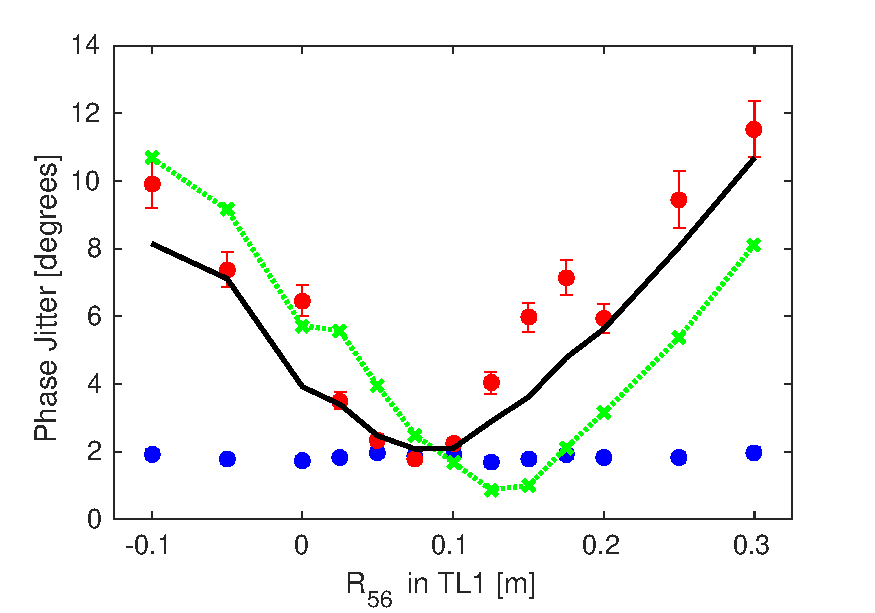
\includegraphics[width=0.8\textwidth]{Figures/propagation/R56ScanGunWiggle_PhaseJitter}
  \caption{Phase jitter downstream (red markers) and upstream (blue markers) for each set of \(R_{56}\) optics used in TL1 during the scan whilst varying the beam energy. The dashed green line shows a simulation of the expected downstream jitter including only the first order \(R_{56}\) effects. The solid black line shows a simulation of the expected downstream phase jitter including the effects of both \(R_{56}\) and \(T_{566}\).}
  \label{f:R56ScanGunWiggle_PhaseJitter}
  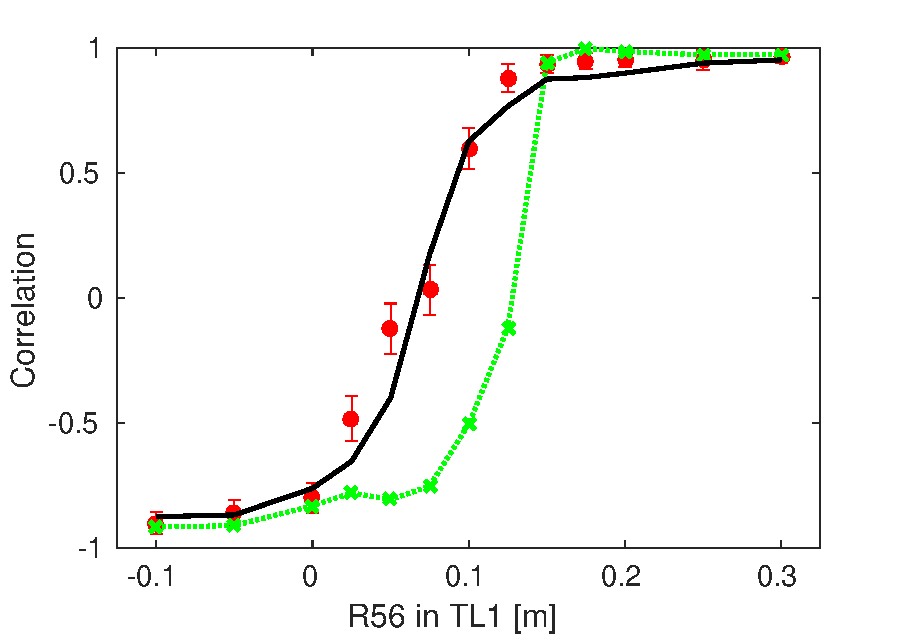
\includegraphics[width=0.8\textwidth]{Figures/propagation/R56ScanGunWiggle_Correl}
  \caption{Upstream-downstream phase correlation (red markers) for each set of \(R_{56}\) optics used in TL1 during the scan whilst varying the beam energy. The dashed green line shows a simulation of the expected correlation including only the first order \(R_{56}\) effects. The solid black line shows a simulation of the expected correlation including the effects of both \(R_{56}\) and \(T_{566}\).}
  \label{f:R56ScanGunWiggle_Correl}
\end{figure}

\begin{figure}
  \centering
  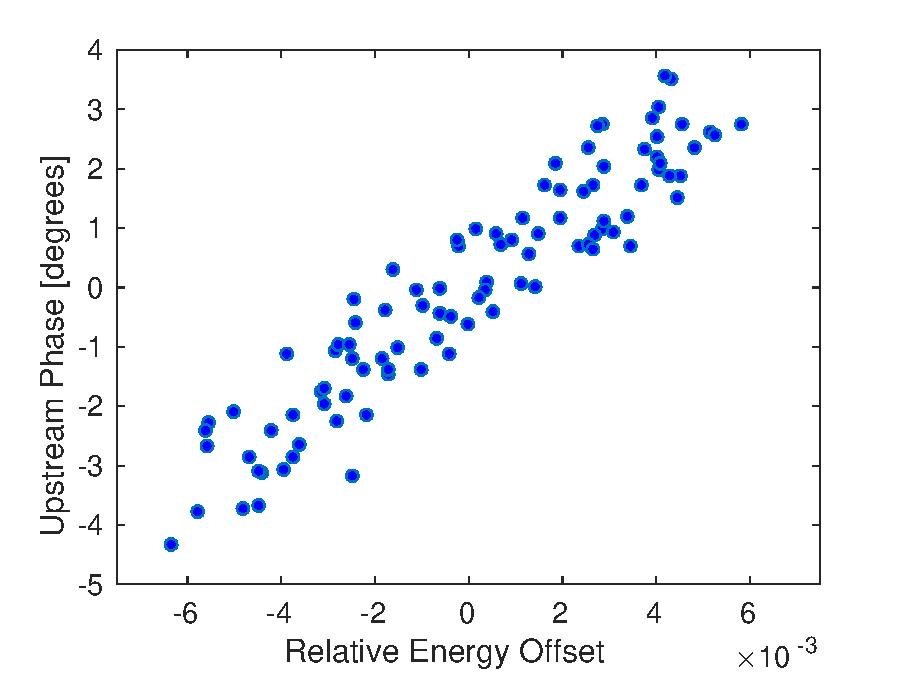
\includegraphics[width=0.8\textwidth]{Figures/propagation/R56ScanGunWiggle_UpEnCorr}
  \caption{Upstream phase-energy correlation whilst varying the beam energy, and with the \(R_{56}=-0.1\)~m optics in TL1.}
  \label{f:R56ScanGunWiggle_UpEnCorr}
\end{figure}

The upstream-downstream phase correlation during the scan is shown in Figure~\ref{f:R56ScanGunWiggle_Correl}. As the correlation between the upstream phase and the beam energy is greatly increased as a result of varying the beam energy as previously discussed, there is no longer a clear singular peak in the upstream-downstream phase correlation during the scan. Instead, the correlation quickly flips between a highly correlated state and a highly anti-correlated state. This is effect was previously seen in Figure~\ref{f:corrVsR56_CTENCorr} as a consequence of the \(R_{56}\) equations derived in Section~\ref{ss:r56Equations}. The actual upstream-downstream phase correlation during the scan is in good agreement with the simulation including the effects of \(T_{566}\) (again with an assumed mean energy offset of \(-2\times10^{-3}\)). The optimal \(R_{56}\) for the phase propagation in terms of the upstream-downstream phase correlation is in the region around \(R_{56}=0.175\)~m in TL1. However, for these \(R_{56}\) values the downstream phase jitter is much larger than the upstream phase jitter due to the effects of the upstream phase-energy correlation and \(T_{566}\) in the high energy jitter conditions during the scan. This makes it more difficult to precisely define the best \(R_{56}\) optics to use based on the results of a scan of this type alone.




\subsubsection{Phase Along the Pulse}

As well as the mean phase it is interesting to look at the effect of varying the \(R_{56}\) on the phase along the pulse. To understand differences in the downstream phase along the pulse it is important to know the properties of the beam energy along the pulse during the \(R_{56}\) scan. Figures~\ref{f:R56ScanGunWiggle_MeanEnergyAlong}~and~\ref{f:R56ScanGunWiggle_EnergyJitterAlong} show typical examples of the mean energy and the energy jitter along the pulse. During this scan the mean beam energy was constantly varied about its initial value, as noted previously. This has no effect on the mean beam energy along the pulse, but does increase the energy jitter along the pulse. The relative beam energy offset along the pulse (Figure~\ref{f:R56ScanGunWiggle_MeanEnergyAlong}) varies by \(3.5\times10^{-3}\) peak-to-peak. The energy jitter along the pulse varies betwen \(4\times10^{-3}\) and \(3\times10^{-3}\), with better stability towards the end of the pulse.

\begin{figure}
  \centering
  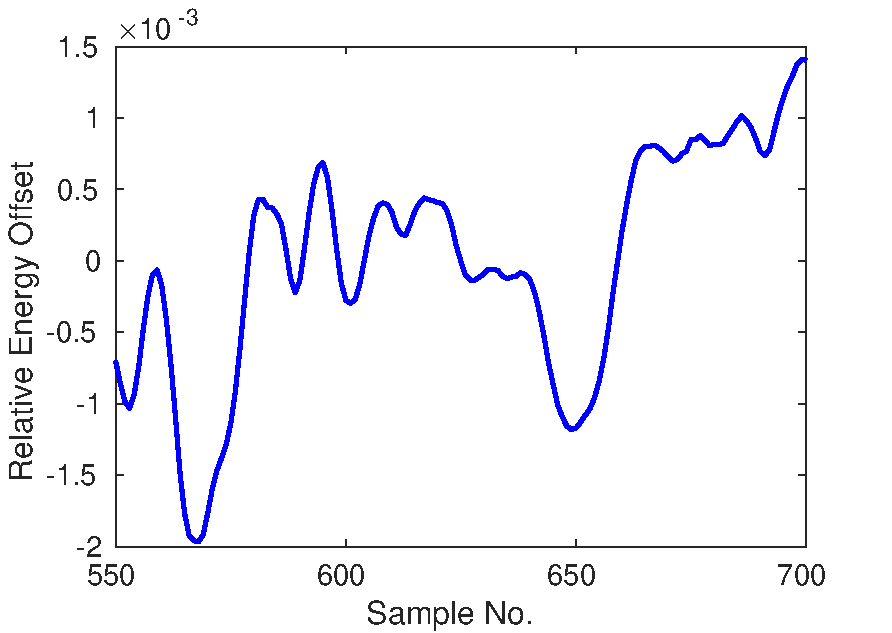
\includegraphics[width=0.8\textwidth]{Figures/propagation/R56ScanGunWiggle_MeanEnergyAlong}
  \caption{Typical example of variations in the mean energy along the pulse during the \(R_{56}\) scan.}
  \label{f:R56ScanGunWiggle_MeanEnergyAlong}
\end{figure}

\begin{figure}
  \centering
  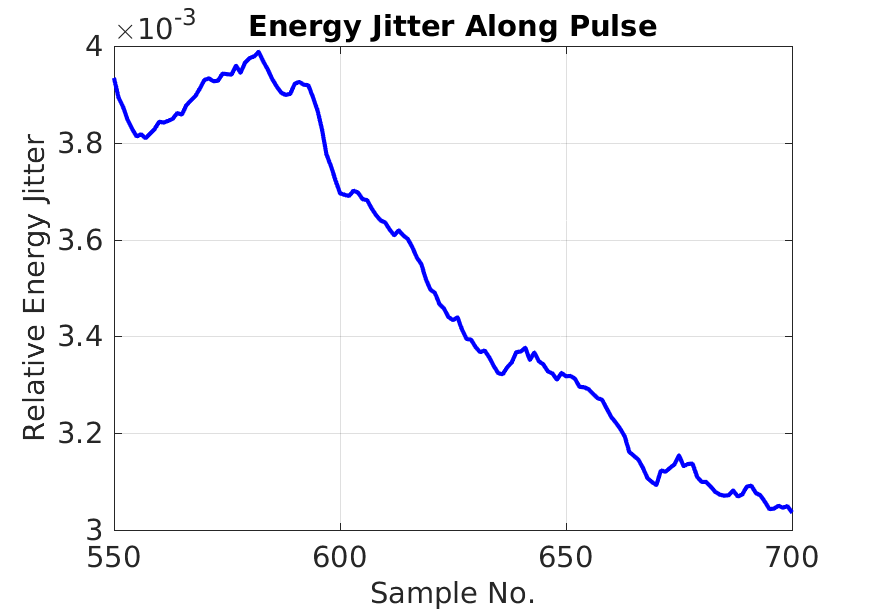
\includegraphics[width=0.8\textwidth]{Figures/propagation/R56ScanGunWiggle_EnergyJitterAlong}
  \caption{Typical energy jitter along the pulse during the \(R_{56}\) scan, amplified by varying the mean beam energy during the scan.}
  \label{f:R56ScanGunWiggle_EnergyJitterAlong}
\end{figure}

Figure~\ref{f:r56Scan_meanPhaseAlong} shows the mean phase along the pulse for each \(R_{56}\) setting in TL1 during the scan. Any difference in the mean (rather than the jitter) along the pulse with the \(R_{56}\) value should originate from variations in the mean energy along the pulse. If the energy along the pulse was constant changing the \(R_{56}\) would only affect the phase jitter and would not change the mean pulse shape. The clear change in certain features along the pulse in the downstream phase is therefore an indication of energy variations in these regions. Perhaps the best example of this is the oscillation around a time of 800~ns, where the phase is flat close to the optimal \(R_{56}\) value of 0.1~m but swings upwards when a negative \(R_{56}\) in TL1 is used or downards for \(R_{56}\) values above 0.15~m.

\begin{figure}
  \centering
  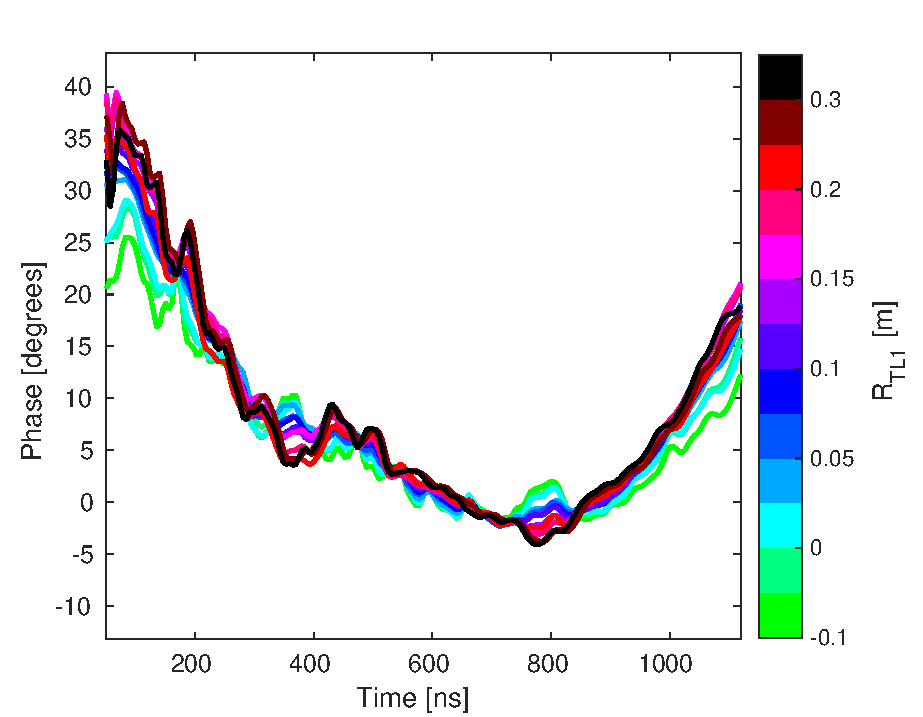
\includegraphics[width=0.8\textwidth]{Figures/propagation/r56Scan_meanPhaseAlong}
  \caption{Mean downstream phase along the pulse for all sets of \(R_{56}\) optics used in TL1 during the scan whilst varying beam energy.}
  \label{f:r56Scan_meanPhaseAlong}
\end{figure}

The difference between the phase along the pulse for two different settings of \(R_{56}\) in TL1 should be proportional to the beam energy along the pulse. Figure~\ref{f:r56Scan_comparisonPhaseEnergy} plots the difference between the \(R_{56}\)~=~+0.3~m optics and the roughly optimal \(R_{56}\)~=~+0.175~m optics, and compares this to the beam energy along the pulse. Both lines are mean subtracted and normalised to give equivalent amplitudes in arbitrary units. Overall, the differences in phase along the pulse resulting from using non-optimal R56 in TL1 are very well matched with the energy variation along the pulse, as expected. 

\begin{figure}
  \centering
  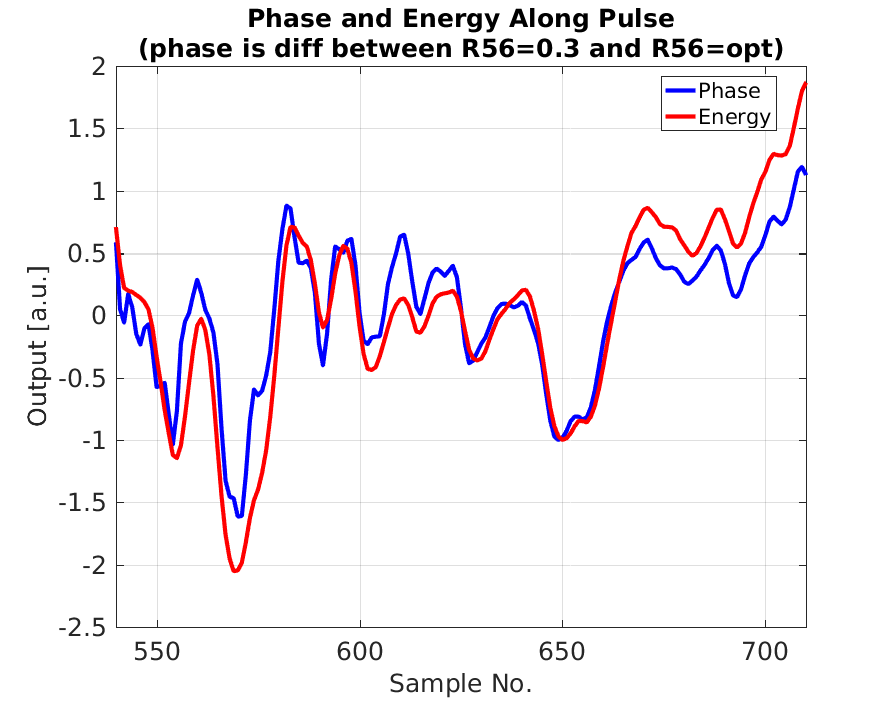
\includegraphics[width=0.8\textwidth]{Figures/propagation/r56Scan_comparisonPhaseEnergy}
  \caption{Difference between the mean downstream phase along the pulse with \(R_{56} = 0.3\)~m and 0.175~m in TL1 (blue) compared to the beam energy along the pulse (red).}
  \label{f:r56Scan_comparisonPhaseEnergy}
\end{figure}

Figure~\ref{f:R56ScanGunWiggle_JitterAlong} shows the downstream phase jitter along the pulse for each \(R_{56}\) optics in TL1 used during the scan. Like the mean phase jitter, the jitter along the pulse is lowest for \(R_{56}\) values between 0.05~m and 0.1~m in TL1 (blue). Lower \(R_{56}\) values (green) and higher \(R_{56}\) values (purple, red and black) give higher jitter. Close to the optimal \(R_{56}\) value many of the variations in jitter along the pulse are reduced, although in all cases some features remain.

\begin{figure}
  \centering
  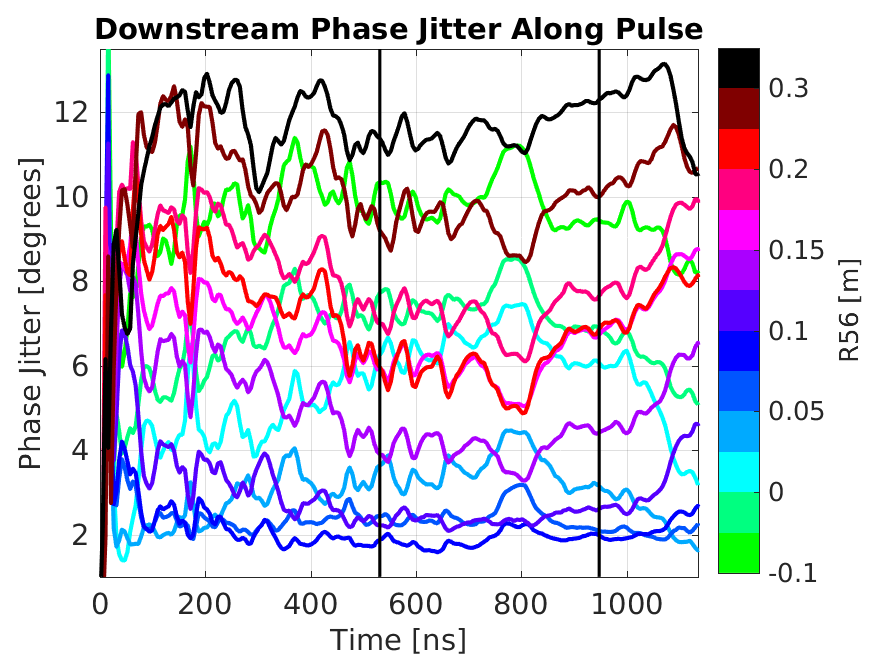
\includegraphics[width=0.8\textwidth]{Figures/propagation/R56ScanGunWiggle_JitterAlong}
  \caption{Downstream phase jitter along the pulse for each set of optics used in TL1 during the \(R_{56}\) scan whilst varying beam energy.}
  \label{f:R56ScanGunWiggle_JitterAlong}
\end{figure}

Differences in the phase jitter along the pulse between two different \(R_{56}\) optics in TL1 should also be related to the beam energy. One might expect the features in the downstream phase jitter along the pulse to match the shape of the variations in energy jitter along the pulse shown previously. Figure~\ref{f:stdPhaseVsStdEnergyAlong} compares the difference in phase jitter along the pulse for the \(R_{56} = 0.075\)~m and \(R_{56} = -0.1\)~m optics to the energy jitter along the pulse. There is no clear similarity between the two. In Figure~\ref{f:stdPhaseVsMeanEnergyAlong} the phase jitter along the pulse is compared to the mean energy along the pulse instead. In this case most of the features in the downstream phase jitter are also present in the energy along the pulse. Static variations in the mean energy along the pulse are therefore more critical for the phase propagation than differences in energy jitter along the pulse. This is true even in the conditions used in this scan,  in which the energy jitter was artificially increased.

\begin{figure}
  \centering
  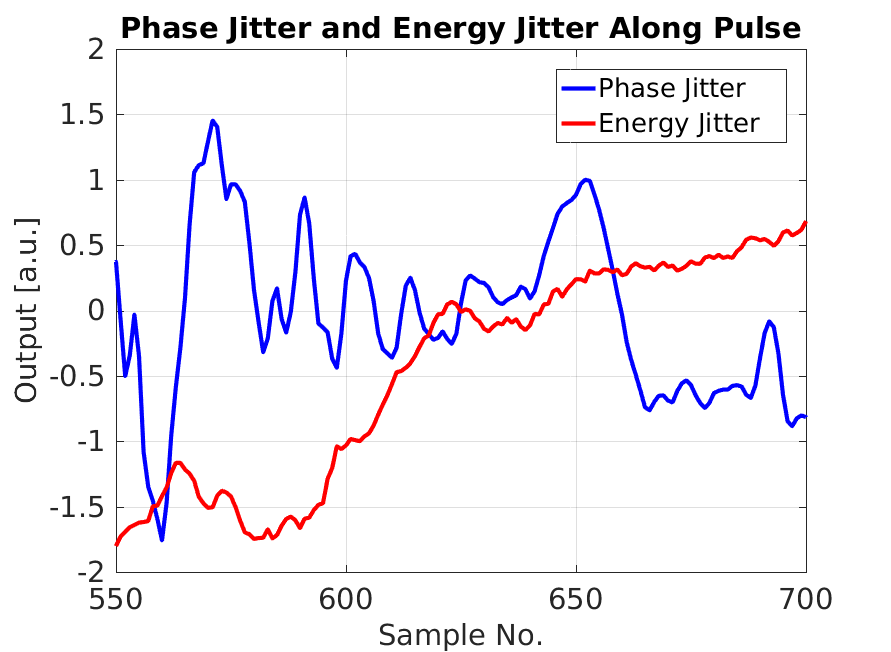
\includegraphics[width=0.8\textwidth]{Figures/propagation/stdPhaseVsStdEnergyAlong}
  \caption{Difference between the downstream phase jitter along the pulse with \(R_{56} = 0.3\)~m and 0.175~m in TL1 (blue) compared to the energy jitter along the pulse (red).}
  \label{f:stdPhaseVsStdEnergyAlong}
\end{figure}

\begin{figure}
  \centering
  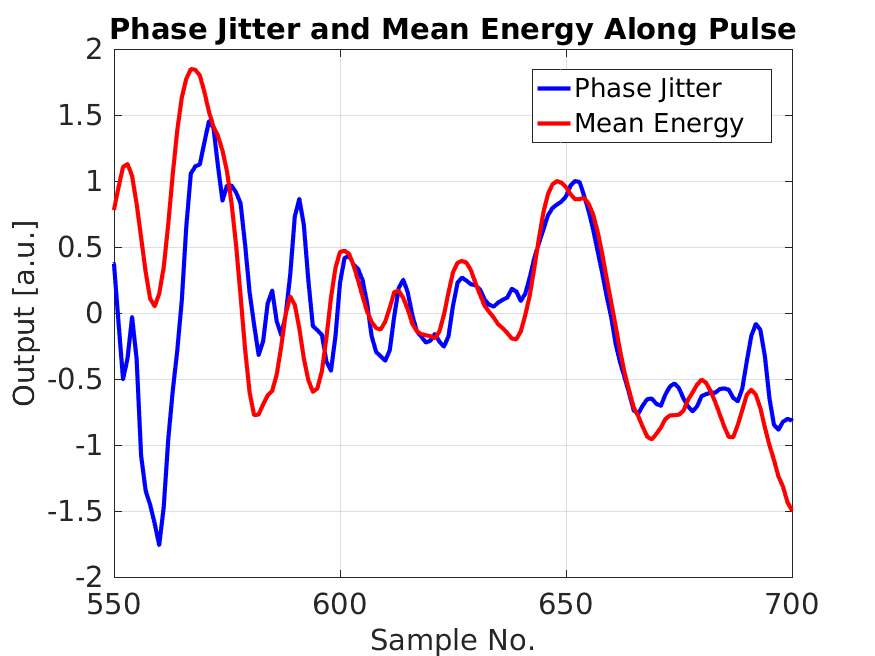
\includegraphics[width=0.8\textwidth]{Figures/propagation/stdPhaseVsMeanEnergyAlong}
  \caption{Difference between the downstream phase jitter along the pulse with \(R_{56} = 0.3\)~m and 0.175~m in TL1 compared to the mean beam energy along the pulse (red).}
  \label{f:stdPhaseVsMeanEnergyAlong}
\end{figure}

\subsection{Mitigation of Higher Order Dependencies}
\label{ss:t566Mitigation}

The first order energy dependent effects on the downstream phase due to the \(R_{56}\) in TL2 have largely been successfully removed by adding positive \(R_{56}\) to the TL1 line. If necessary, further improvements could be made by creating further sets of TL1 optics in smaller \(R_{56}\) steps. Although the higher order energy dependent effects due to \(T_{566}\) have been identified they are more difficult to remove or reduce. To remove the effect completely new optics would have to be matched with constraints included to zero the \(T_{566}\) value between the usptream and downstream phase monitors. This would likely require the use of sextupoles, which are typically left unpowered at CTF3 due to difficulties in commissioning optics that include them \cite{piotrPriv}. It also depends on the accuracy of the MADX model of CTF3 to second order, although the result in Figure~\ref{f:R56ScanGunWiggle_T566Fit} is promising in this regard, at least in the \(R_{56}\) range of interest.

Alternatively, the second order effects can be reduced by decreasing the energy jitter and variaitions along the pulse at CTF3. Many improvements have recently been made at CTF3 to achieve this via the implementation of several new feedbacks [REF LukasIPAC]. New feedbacks on the phases of each klystron in the CTF3 injector as well as on the beam gun current are now routinely in operation, and these have already improved the mean energy jitter to \(0.5\times10^{-3}\) on short time scales of several minutes, or \(0.8\times10^{-3}\) on longer time scales. Hardware changes and further improvements to the implementation of these feedbacks should allow the mean energy stability to be improved further in 2016.

In addition, although they are not yet run online in normal operation, new feedbacks have also been implemented and commissioned that can smooth energy variations along the pulse, or directly smooth the upstream phase along the pulse itself. The energy flattening feedback [REF Tobias] varies the waveform of the last klystron in the CTF3 linac based on the measurement of the same dispersive BPM used to measure the beam energy in this chapter --- CT.0608 in TL1. This flattens the energy along the pulse by varying the energy gain along the pulse in the last accelerating structure. In addition, prior to the best phase propagation conditions currently achieved (presented in the next section) a similar feedback was used to smooth features in the upstream phase along the pulse by varying the waveform of the first klystron in the CTF3 linac [REF Davide]. Feedbacks of this type will be critical to be able to improve the PFF performance in 2016.

\begin{figure}
  \centering
  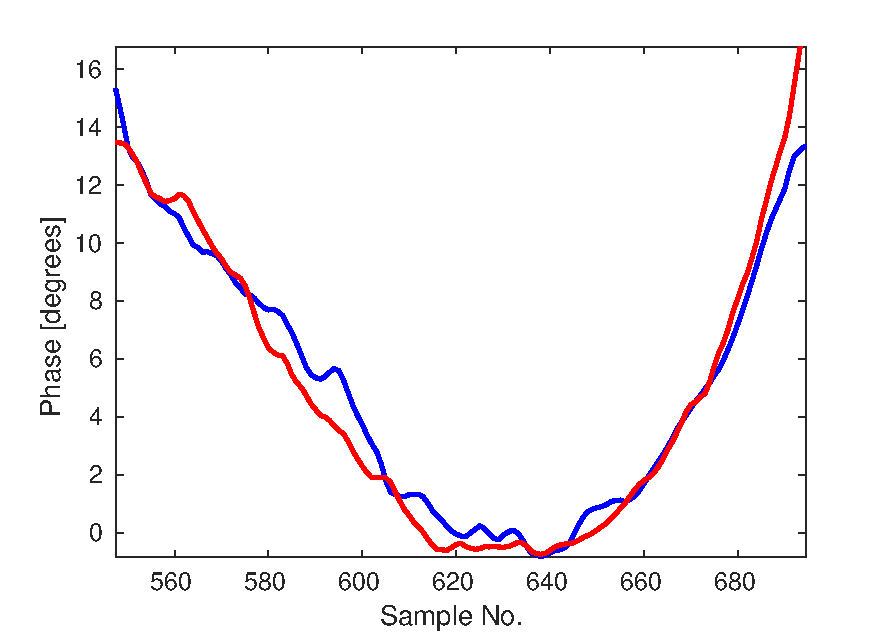
\includegraphics[width=0.8\textwidth]{Figures/propagation/beforeAfterDavideFlatten}
  \caption{Effect of feedback used to smooth variations along the upstream phase (initial upstream phase in blue, and after applying the feedback in red).}
  \label{f:beforeAfterDavideFlatten}
\end{figure}


\newsection{bestPhaseProp}{Best Phase Propagation}

This section summarises the best phase propagation conditions that have been achieved to date after the extensive work to identify and reduce the energy dependence of the downstream phase. The results shown here are taken from the same dataset with which the best PFF results were achieved, presented later in Section~\ref{s:jitterRecord}. At this time the \(R_{56} = +0.1\)~m optics was used in TL1. The achieved conditions are a remarkable improvement compared to the original status presented in Section~\ref{s:origJitter}. The reproducibility of these conditions is discussed in the context of the PFF results in Section~\ref{s:longPFF}.

\subsubsection{Mean Phase}

The best phase propagation conditions are achieved when the correlation between the phase and the beam energy is the same upstream and downstream. Figure~\ref{f:bestProp_enCorr} shows the correlation of the usptream and downstream phase with the beam energy. With the optimised conditions almost all correlation between the downstream phase and the beam energy is removed, with a correlation of \(0.2\pm0.1\). This agrees with the upstream-downstream phase correlation of \(0.1\pm0.1\) within error bars.

\begin{figure}
  \centering
  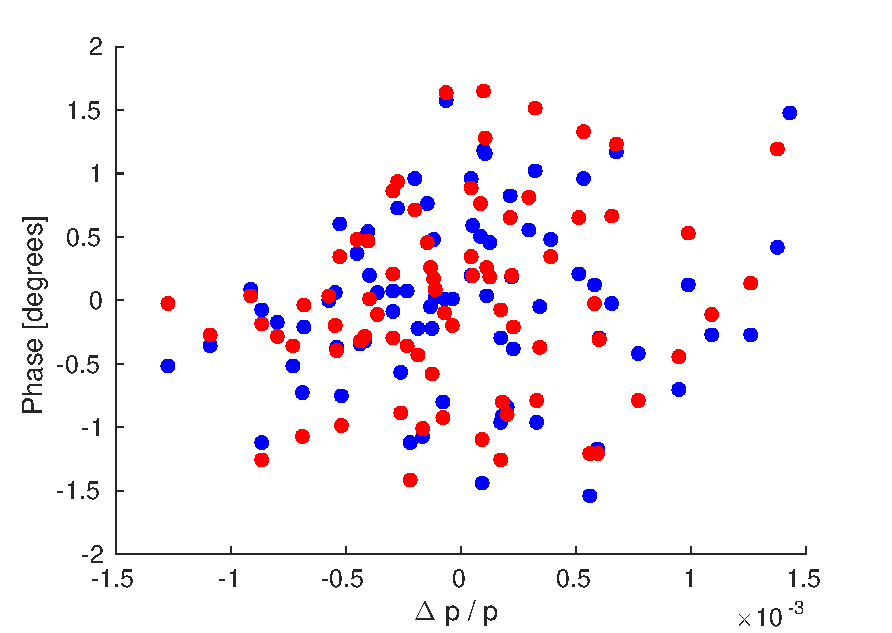
\includegraphics[width=0.8\textwidth]{Figures/propagation/bestProp_enCorr}
  \caption{Upstream (blue) and downstream (red) phase-energy correlation with optimised phase propagation.}
  \label{f:bestProp_enCorr}
\end{figure}

Figure~\ref{f:bestProp_meanPhase} shows that all drifts in the upstream phase are also present downstream, and that the usptream and downstream mean phase jitters are also the same within errors bars --- \(0.69\pm0.06^\circ\) upstream and \(0.74\pm0.06^\circ\) downstream. The standard deviation of the residuals between the upstream and downstream phase is \(0.27\pm0.02^\circ\), which corresponds to below 0.2 degrees actual beam jitter between the two phases when the phase monitor resolution is taken in to account. The correlation between the mean upstream and downstream phase is \(93\pm4\%\), as shown in Figure~\ref{f:bestProp_meanCorr}. This is very close to the targeted \(97\%\) that would make a reduction in downstream jitter to \(0.2^\circ\) possible with the PFF system.

\begin{figure}
  \centering
  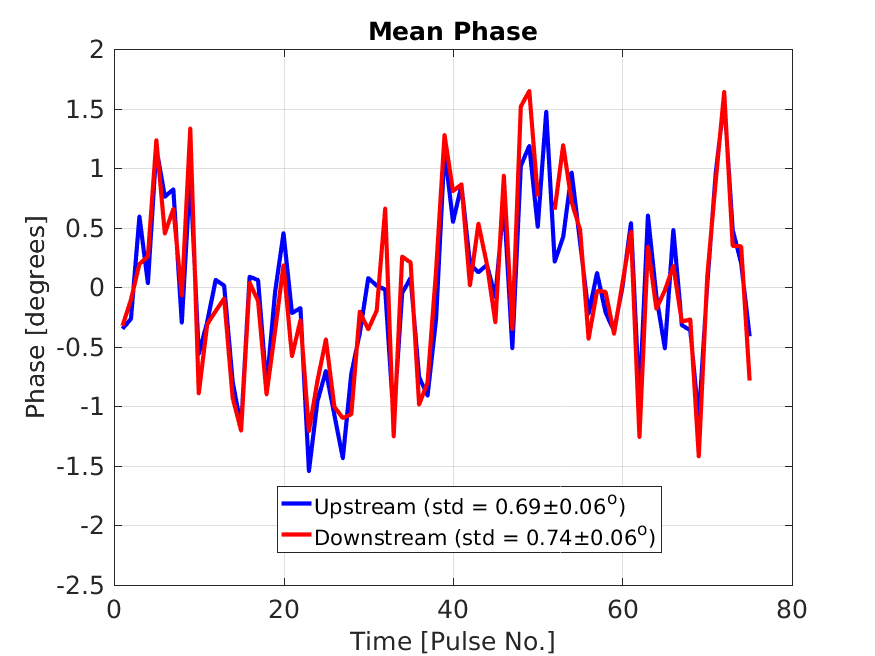
\includegraphics[width=0.8\textwidth]{Figures/propagation/bestProp_meanPhase}
  \caption{Mean phase vs. time upstream (blue) and downstream (red) with optimised phase propagation.}
  \label{f:bestProp_meanPhase}
\end{figure}

\begin{figure}
  \centering
  \includegraphics[width=0.8\textwidth]{Figures/propagation/bestProp_meanCorr}
  \caption{Upstream-downstream phase correlation with optimised phase propagation. The black line shows a linear fit to the data (blue markers).}
  \label{f:bestProp_meanCorr}
\end{figure}

\subsubsection{Phase Along Pulse}

Figure~\ref{f:bestProp_meanAlong} compares the phase along the pulse upstream and downstream in the optimal conditions. For reference, the mean phases presented above were calculated in the region between 530~ns and 950~ns. This is the flat central part of the pulse where the PFF system can provide the maximum reduction in phase jitter, as seen in Section~\ref{s:jitterRecord}. The overall agreement in shape between the upstream and downstream phase is excellent, with almost all energy dependent features also removed from the mean downstream phase along the pulse. There are still some remaining differences in shape, particularly at the start and end of the pulse before and after the 530--950~ns range.

\begin{figure}
  \centering
  \includegraphics[width=0.8\textwidth]{Figures/propagation/bestProp_meanAlong}
  \caption{Phase along the pulse upstream (blue) and downstream (red) with optimised phase propagation.}
  \label{f:bestProp_meanAlong}
\end{figure}

By viewing the phase jitters and correlations along the pulse the remaining areas for improvement start to become apparent. In Figure~\ref{f:bestProp_jitAlong}, showing the phase jitter along the pulse, it is clear that the start of the pulse is less stable. For times between 100~ns and 600~ns the downstream phase jitter is as much as 60\% larger than the upstream phase jitter.  However, there is a 400~ns portion of the pulse where the downstream phase jitter has been successfully reduced to the level of the usptream phase jitter. The best PFF results can be expected in this region.

\begin{figure}
  \centering
  \includegraphics[width=0.8\textwidth]{Figures/propagation/bestProp_jitAlong}
  \caption{Phase jitter along the pulse upstream (blue) and downstream (red) with optimised phase propagation.}
  \label{f:bestProp_jitAlong}
\end{figure}

The upstream-downstream phase correlation along the pulse, in Figure~\ref{f:bestProp_corrAlong}, is at the same level as the mean phase correlation in the region between 450~ns and 650~ns. However, there are also parts of the pulse where the upstream-downstream phase correlation is greatly reduced -- to 55\% at 300~ns and 70\% at 700~ns, for example. Differences earlier in the pulse are not critical for the PFF system, but the feature at 700~ns is in the area where the correction is attempted.

By comparing the upstream-downstream correlation along the pulse to the correlations with energy along the pulse, in Figure~\ref{f:bestProp_enCorrAlong}, the problem becomes clear. Due to energy variations along the pulse and the effect of higher order energy dependencies, as previously discussed, the phase propagation can not be optimised across the full pulse length. As a result there are parts of the pulse where the downstream phase-energy correlation is still high, up to 75\%. Areas where there is a large difference between the upstream phase-energy correlation and the downstream phase-energy correlation correspond to regions of degraded upstream-downstream phase correlation in Figure~\ref{f:bestProp_jitAlong}. This is the key area where improvements are needed in 2016 in order to further improve the PFF performance.

\begin{figure}
  \centering
  \includegraphics[width=0.8\textwidth]{Figures/propagation/bestProp_corrAlong}
  \caption{Upstream-downstream phase correlation along the pulse with optimised phase propagation.}
  \label{f:bestProp_corrAlong}
  \includegraphics[width=0.8\textwidth]{Figures/propagation/bestProp_enCorrAlong}
  \caption{Upstream (blue) and downstream (red) phase-energy correlation along the pulse with optimised phase propagation.}
  \label{f:bestProp_enCorrAlong}
\end{figure}

\newsection{otherJitterSources}{Possible Other Sources of Phase Jitter}

The energy related effects on the downstream phase have been the main focus of attempts to improve the phase propagation for the PFF system, and as shown in the previous section this by itself has lead to upstream-downstream correlations in excess of 90\% to be achieved at CTF3. Further optimisations will be needed to achieve the \(97\%\) correlation required to achieve the CLIC target of 0.2 degrees phase jitter with the PFF prototype, however. This can partly come from further improvements of the CTF3 injector setup and stability in 2016, which will help to reduce any remaining effects from \(T_{566}\) by reducing beam energy jitter, drifts and variations along the pulse. At correlations above \(90\%\) any remaining small differences in the performance of the upstream and downstream phase monitors may also become significant, but this has been adressed in Chapter~\ref{c:phaseMons} so will not be discussed again here.

Preliminary measurements have been taken to investigate whether there may be any other instabilities at CTF3, apart from energy jitter, that can change the downstream phase and reduce the upstream-downstream phase correlation. The most likely culprits are devices between the upstream and downstream phase monitors that have a strong effect on the beam orbit. Any change in beam orbit can change the path length between the upstream and downstream phase monitors, and thus shift the downstream phase with respect to the upstream phase. The main elements for which this could be significant include the dipoles in TL1 and the combiner ring, as well as the two septum magnets used  at the combiner ring injection and extraction. Instabilities on the power supplies for one of these devices could be an additional source of uncorrelated downstream phase jitter.

The current applied from the power supplies for each of these devices has been varied to determine their effect on the downstream phase. In some cases one power supply drives multiple devices, meaning these devices can not be changed independently from each other and any jitter in their strengths should be correlated (assuming the jitter source is the power supply, rather than a separate issue with the device itself). There are four power supplies that control the strength of the devices of interest in the following groups:
\begin{itemize}
\item \textbf{Power supply 1:} The first (CT.0540) and last (CT.0710) dipole in TL1.
\item \textbf{Power supply 2:} The second (CT.0630) and third (CT.0670) dipole in TL1.
\item \textbf{Power supply 3:} The combiner ring injection and extraction setpa.
\item \textbf{Power supply 4:} All combiner ring dipoles.
\end{itemize}
Figures~\ref{f:tl1540}--\ref{f:crBends} show the effect of changing each of these power supplies on the downstream phase. A linear fit to the response is also shown. Where the response is non-linear (for the combiner ring dipoles, for example) the fit is only applied in the central region around the nominal device setting, to give an approximate gradient that is relevant for small offsets. In some cases, particularly for the 540/710 dipoles in TL1, the phase dependence is not clear. In all cases the goal is to determine whether there is an effect that may be significant for the PFF system, which can then be investigated further later, rather than quoting precise numbers.

%\begin{figure}
%  \centering
%  \includegraphics[width=0.8\textwidth]{Figures/propagation/tl1540}
%  \caption{Phase vs. strength of first and last dipole in TL1 (CT.0540 and CT.0710).}
%  \label{f:tl1540}
%\end{figure}

\begin{figure}
  \centering
  \includegraphics[width=0.8\textwidth]{Figures/propagation/tl1670}
  \caption{Downstream phase vs. strength (power supply current) of the first and last dipole in TL1 (CT.0630 and CT.0670).}
  \label{f:tl1670}
\end{figure}

%\begin{figure}
%  \centering
%  \includegraphics[width=0.8\textwidth]{Figures/propagation/crSeptum}
%  \caption{Phase vs. strength of the combiner ring injection and extraction septum magnets.}
%  \label{f:crSeptum}
%\end{figure}

\begin{figure}
  \centering
  \includegraphics[width=0.8\textwidth]{Figures/propagation/crBends}
  \caption{Downstream phase vs. strength (power supply current) of the combiner ring dipoles).}
  \label{f:crBends}
\end{figure}

The power supplies at CTF3 give a relative stability in the supplied current of approximately \(10^{-4}\). Assuming this stability the effect of each device on the downstream phase jitter can be determined by using the fitted gradients from the plots previously shown and the known current setting for each device. These values are summarised in Table~\ref{t:otherJitSources}. By far the strongest potential source of phase jitter appears to be the middle two dipoles in TL1 (CT.0630 and CT.0670), which by themselves could contribute \(0.17\pm0.03\) degrees phase jitter. The explanation for these two dipoles having a much larger effect on the phase than the first and last dipole in TL1 is not known and will need to be verified by repeated measurements and checks of the expected response in the CTF3 MADX model. The combiner ring devices contribute roughly 5 times less phase jitter than the CT.0630 and CT.0670 dipoles. Combining the estimated phase jitters resulting from these devices in qudrature gives an overall contribution of \(0.18\pm0.03^\circ\) additional downstream phase jitter.

\begin{table}
  \begin{center}
    \begin{tabular}{| c c c c |}
	   \hline
       Device & Current & Fit Gradient & Estimated Phase Jitter \\ \hline
       TL1 540/710 Dipoles & 133~A & \(-0.4\pm0.3^\circ\)/A & \(0.005\pm0.004^\circ\)\\
       TL1 630/670 Dipoles & 164~A & \(10\pm2^\circ\)/A & \(0.17\pm0.03^\circ\)\\
       CR Septa & 890~A &  \(-0.5\pm0.1^\circ\)/A & \(0.05\pm0.01^\circ\)\\
       CR Dipoles & 156~A & \(1.8\pm0.7^\circ\)/A & \(0.03\pm0.01^\circ\)\\ \hline 
    \end{tabular}
    \caption{Current setting, dependence of the downstream phase on the current and estimated contribution to downstream phase jitter for the dipoles and septa in TL1 and the combiner ring.}
  	\label{t:otherJitSources}
  \end{center}
\end{table}

Modelling the downstream phase as \(\phi_d = \phi_u + x\), where \(x\) is a generic additional source of jitter, the downstream jitter and upstream-downstream phase correlation are given by:
\begin{eqnarray}
\sigma_d = \sqrt{\sigma_u^2 + \sigma_x^2} \\
\rho_{ud} = \frac{\sigma_u}{\sigma_d}
\end{eqnarray}
These are simplified forms of the equations in Section~\ref{ss:r56Equations} in the case where the additional jitter source is uncorrelated with the upstream phase (which is not the case for the energy dependent phase jitter). Assuming an initial upstream phase jitter of \(0.8^\circ\) plus a \(\sigma_x = 0.18^\circ\) source of jitter resulting from the power supply stabilities previously discussed, the downstream phase jitter is increased slightly to \(0.82^\circ\) and the upstream-downstream phase correlation reduced to \(98\%\). This by itself does not prevent the PFF system from theoretically achieving \(0.2^\circ\) phase jitter, for which \(\rho_{ud} = 0.97\) is required. However, in combination with the effects of \(R_{56}\), \(T_{566}\) and the phase monitor resolution, each of which can individually reduce the correlation to 0.97 or below depending on the conditions, this highlights that the \(0.2^\circ\) target will be very difficult to achieve with the PFF prototype at CTF3.
